\documentclass[conference, onecolumn, a4, 12pt]{IEEEtran}
\IEEEoverridecommandlockouts
% The preceding line is only needed to identify funding in the first footnote. If that is unneeded, please comment it out.
\usepackage{cite}
\usepackage{amsmath,amssymb,amsfonts}
\usepackage{algorithmic}
\usepackage{graphicx}
\usepackage{textcomp}
\usepackage{xcolor}
\pagenumbering{arabic}
\def\BibTeX{{\rm B\kern-.05em{\sc i\kern-.025em b}\kern-.08em
    T\kern-.1667em\lower.7ex\hbox{E}\kern-.125emX}}
\newcommand\tab[1][1cm]{\hspace*{#1}}
\renewcommand{\familydefault}{\rmdefault}

\begin{document}
\title{Using neural networks to generate test cases using BDD specifications}

\author{
\IEEEauthorblockN{Nugawela, N. P. S. C.}
\textit{Index No.} 189337J \\
\IEEEauthorblockA{\textit{Department of Computer Science and Engineering} \\
\textit{University of Moratuwa}\\
Moratuwa, Sri Lanka \\
chaparanga.18@cse.mrt.ac.lk}\\

Supervised by Dr. U. Thayasivam \\
\IEEEauthorblockA{\textit{Department of Computer Science and Engineering} \\
\textit{University of Moratuwa}\\
Moratuwa, Sri Lanka \\
rtuthaya@cse.mrt.ac.lk}\\

CS5999PGP PG Diploma Project Report	\\
Department of Computer Science and Engineering\\
January 2019
}

\maketitle
\pagebreak
\setcounter{page}{1}
\pagestyle{plain}

\begin{center}
\textbf{Declaration}\newline
I declare that this is my own work and this PG Diploma Project Report does not incorporate without acknowledgement any material previously submitted for a Degree or Diploma in any other University or institute of higher learning and to the best of my knowledge and belief, it does not contain any material previously published or written by another person except where the acknowledgement is made in the text.\newline
Also, I hereby grant to University of Moratuwa the non-exclusive right to reproduce and distribute my thesis, in whole or in part in print, electronic or other medium. I retain the right to use this content in whole or part in future works.\newline
\end{center}

\_\_\_\_\_\_\_\_\_\_\_\_\_\_ \tab\tab\tab\tab\tab\tab\tab \_\_\_\_\_\_\_\_\_\_\_\_\_\_\newline\newline
N. P. S. C. Nugawela \tab\tab\tab\tab\tab\tab\tab Date \newline

I certify that the declaration above by the candidate is true to the best of my knowledge and that this project report is acceptable for evaluation for the CS5999PGP PG Diploma Project.\newline\newline

\_\_\_\_\_\_\_\_\_\_\_\_\_\_ \tab\tab\tab\tab\tab\tab\tab \_\_\_\_\_\_\_\_\_\_\_\_\_\_\newline\newline
Dr. Uthayan Thayasivam \tab\tab\tab\tab\tab\tab\tab Date

\pagebreak

\begin{center}
\textbf{Acknowledgement}
\end{center}
My utmost gratitude and appreciation in making this project a success goes to my family who were very patient and supportive towards me and my supervisor, Dr. Uthayan Thayasivam, who advised me greatly in the preparation of this project and all the wonderful people who have furthered the knowledge in the domains of Computer Science that facilitated this project.

\pagebreak

\tableofcontents
\pagebreak

\begin{abstract}
Testing is an integral part of software development. In recent times, ideologies such as TDD (Test Driven Development) and BDD (Behaviour Driven Development) have become popular. Here, we will be looking at BDD and how we can improve upon the current methods of implementing BDD testing and automating the process of impelmenting tests based on BDD. We aim to use neural network based solutions to achieve this task.  
\end{abstract}

\begin{IEEEkeywords}
TDD (Test Driven Development), BDD (Behaviour Driven Development), GAN (Generative Adversarial Network), NLP (Natural Language Processing), POC (Proof Of Concept), SUT (System Under Test), GUI (Graphical User Interface), RNN (Recurrent Neural Network), Long Short Term Memory (LSTM), Software Engineering (SE), Online Judge (OJ) 
\end{IEEEkeywords}

\section{Introduction}
The writing of tests for software projects has become very important in the modern era of software development. BDD has become a new trend wherein the test case is written in a user readable manner. The language used to specify the test cases is called Gherkin. Gherkin follows a simple format where a few select keywords are used to specify full user requirements.\cite{a1} The primary keywords are,
\begin{enumerate}
	\item Feature
	\item Example (or Scenario)
	\item Given, When, Then, And, But (steps)
	\item Background
	\item Scenario Outline (or Scenario Template)
	\item Examples
\end{enumerate}

There are some secondary keywords as well, which are,

\begin{enumerate}
	\item " " " (Doc Strings)
	\item | (Data Tables)
	\item @ (Tags)
	\item \# (Comments)
\end{enumerate}

Now we shall delve into the keywords in detail \cite{a1}.
\subsection{Feature}
The purpose of the Feature keyword is to provide a high-level description of a software feature, and to group related scenarios.

The first primary keyword in a Gherkin document must always be Feature, followed by a : and a short text that describes the feature.

You can add free-form text underneath Feature to add more description \cite{a1}.

\subsection{Example}
This is a concrete example that illustrates a business rule. It consists of a list of steps. The keyword Scenario is a synonym of the keyword Example.You can have as many steps as you like, it is recommended that you keep the number at 3-5 per scenario. If they become longer than that, they lose their expressive power as specification and documentation.\newline
In addition to being a specification and documentation, a scenario is also a test. As a whole, your scenarios are an executable specification of the system.\newline
Examples follow this same pattern, \cite{a1}
\begin{itemize}
	\item Describe an initial context (Given steps)
	\item Describe an event (When steps)
	\item Describe an expected outcome (Then steps)
\end{itemize}

\subsection{Steps}
Each step starts with Given, When, Then, And, or But. Keywords are not taken into account when looking for a step definition. This means you cannot have a Given, When, Then, And or But step with the same text as another step \cite{a1}.

\subsubsection{Given}
Given steps are used to describe the initial context of the system - the scene of the scenario. It is typically something that happened in the past. The purpose of Given steps is to put the system in a known state before the user (or external system) starts interacting with the system (in the When steps). Avoid talking about user interaction in Given’s. If you were creating use cases, Given’s would be your preconditions \cite{a1}.

\subsubsection{When}
When steps are used to describe an event, or an action. This can be a person interacting with the system, or it can be an event triggered by another system.

It’s strongly recommended you only have a single When step per Scenario. If you feel compelled to add more, it’s usually a sign that you should split the scenario up into multiple scenarios \cite{a1}.

\subsubsection{Then}
Then steps are used to describe an expected outcome, or result.

The step definition of a Then step should use an assertion to compare the actual outcome (what the system actually does) to the expected outcome (what the step says the system is supposed to do).

An observation should be on an observable output. That is, something that comes out of the system (report, user interface, message), and not something deeply buried inside it (like a database) \cite{a1}.

\subsubsection{And/But}
If you have several Given’s, When’s, or Thens, you could write: \cite{a1}

\begin{list}{*}{spacing}
	\item Example: Multiple Givens
	\item Given one thing
	\item Given another thing
	\item Given yet another thing
	\item When I open my eyes
	\item Then I should see something
	\item Then I shouldn't see something else
\end{list}

Or, we could make it read more fluidly by writing:  \cite{a1}
\begin{list}{*}{spacing}
	\item Example: Multiple Givens
	\item Given one thing
	\item And another thing
	\item And yet another thing
	\item When I open my eyes
	\item Then I should see something
	\item But I shouldn't see something else
\end{list}

\subsubsection{Background}
Occasionally we will need to repeat the same Given steps in all of the scenarios in a feature.

Since it is repeated in every scenario, this is an indication that those steps are not essential to describe the scenarios; they are incidental details. You can literally move such Given steps to the background, by grouping them under a Background section.

A Background allows you to add some context to the scenarios in the feature. It can contain one or more Given steps.

A Background is run before each scenario, but after any Before hooks. In your feature file, put the Background before the first Scenario.

You can only have one set of Background steps per feature. If you need different Background steps for different scenarios, you’ll need to split them into different feature files.\cite{a1}

\subsubsection{Scenario Outline}
The Scenario Outline keyword can be used to run the same Scenario multiple times, with different combinations of values.

The keyword Scenario Template is a synonym of the keyword Scenario Outline.
A Scenario Outline must contain an Examples (or Scenarios) section. Its steps are interpreted as a template which is never directly run. Instead, the Scenario Outline is run once for each row in the Examples section beneath it (not counting the first header row).\cite{a1}\newline

As you can see, the BDD test cases written in Gherkin have a high amount of structure that can be exploited. Currently, there are frameworks that support the generation and management of BDD test cases from Gherkin specifications. Some of the most popular frameworks used for BDD include,

\begin{itemize}
	\item JDave 
	\item Concordion 
	\item JBehave 
	\item Cucumber
	\item Serenity BDD
	\item SpecFlow   
\end{itemize}

These frameworks are used to map the requirements written in Gherkin style to the test code written in a programming language such as Java, .NET, etc. (Which is known as glue code\cite{a2}) So the programmers must still be ready to write the glue code for the Gherkin test cases. We seek to eliminate the necessity of this particular action.
In this paper we propose a novel method for generating test cases for software projects using recurrent neural networks, GANs, etc.\newline

\section{Motivation}
This project is based on the idea of making a neural network based test case generation. This is a research type project, since this type of code generation is not largely attempted. But, simply implementing a neural network based test code generator is somewhat unappealing. Thia is why this project came to be in its entirety. It integrates the test code generation network into a BDD test case glue code generator. So, it comes along with much more relevance than if it were a simple reasearch project.\newline
Behaviour Driven Development is a practice that is being pushed within the agile practices. Many organizations are now adopting this practice in favour of having a set of comprehensive test documentation that supports multiple tiers within the organization.
\subsection{Making the test writing easy for the developer}
One of the major obstacles in the way of the adoption of BDD is the additional work a developer must put into writing the test cases. While there are frameworks such as Cucumber that support the writing of BDD testing, there is much to be desired. In the case of Cucumber, we have to write the glue code by hand. It would be better if only we had to only write the Gherkin test case specifications.
\subsection{Allowing for greater automation}
Automation is very important for the current development environment as it is required to make deliveries on time to clients. Automating the generation of tests is a good path to take in the pursuit of optimizing the development process.
\subsection{Greater adoption of BDD}
BDD is a very good practice that has many benefits to offer the developers as well as Business Analysts, Managers, etc. So, it s very pleasing to see it being adopted in a greater capacity. So, as I pointed out before as well, the easy implementation of this practice will promote BDD greatly.

There is a huge push geared towards the adoption of BDD, but unfortunately, there are many obstacles that prevent it from being freely and widely adopted. With our work, we seek to make it easy and painless for developers to adopt BDD into their processes.\newline

\section{Literature Review}
We will be using Generative Adversarial Networks (GANs), which are systems of two opposing neural networks that are focused on learning patterns. As I shall elaborate in the oncoming sections, there are many studies that are based on GANs. In those studies, it is usual to see the generation of images from random noise, \cite{b2} image generation using text descriptions, \cite{b5} and much more. Also there have been studies that consider the possibilities of employing GANs to cross domain fields.\cite{b3}\newline
There have not been any previous instances of generating BDD tests using text descriptions and GANs. So what I am suggesting is a novel venture, in terms of GANs.
There has been a code base aware test case generation in "Automatically Generating Tests from Natural Language Descriptions of Software Behavior" by Sunil Kamalakar. The problem description of this paper is as follows; "One weak point of BDD is the “glue code”—programmers are still required to produce program “steps” that correspond to the basic actions described in the natural language scenarios. A number of tools have been developed to make the process of writing this glue code easier and streamlined, and to automatically map phrases in the scenarios onto such steps (typically using regular expressions). However, a manually-written bridge between the scenarios and the programmatic actions that correspond to them is still necessary. The question we put forth is: Can we reduce the burden on programmers by utilizing information in the natural language, so that they don’t have to hand-write the glue code?"\cite{a2} 
The motivations mentioned in this paper are Increase in adoption of BDD, Ubiquitous communication and Reduction in effort, time and cost. These are very similar to our convictions as well. The method proposed in the paper is as follows: "Our solution is to process the user stories written for BDD using state-of-the-art Natural Language Processing (NLP) techniques. Simultaneously, we scan the implementation/skeleton code of the project and capture every required property of the code, using reflection techniques. Once we have these two pieces, we employ a custom probabilistic matcher to map the BDD instructions onto code segments. Finally, based on the results of the probabilistic matcher, the code generator spits out code representing these mappings."\cite{a2}
The thesis by Sunil Kamalakar focuses on his work: \textit{Kirby}, a software tool written in Java, for auto-generating glue code from BDD scenarios. Kirby is capable of auto-generating code for projects implemented in Java. It outputs a specific code format in JUnit, which is a widely used unit testing framework for Java. The reason he has chosen Java is because, it is one of the most popular programming languages in use today, along with being a strictly object-oriented and typed-language.\cite{a2} Our approach differs from this approach as we seek to make the system support multiple programming languages and because we use neural networks.

\subsection{Work flow of Kirby}
Once these user stories are ready, the developer needs to follow the Red-Green-Refactor cycle of TDD. So, he will first use Kirby to generate the glue code, which will be created in Java language as JUnit tests. So, the developer creates a Java project with a folder called “BDD Scenarios”. This folder contains
the feature/story files for the project. When Kirby is run on this input set, it still generates the step definitions in a file called BankAccountSteps.java which is going to be located in the src directory. This file contains a class called BankAccountSteps which has three methods - one for each of the scenarios in the story file. The method names are a camel-cased textual representation of the scenario name. You have to remember that no implementation is still written. The generated step definitions/methods do provide feedback to the developer, that the implementation may not yet exist. The current output of \textit{Kirby} is shown below. When he runs the generated file as a JUnit test, it will fail with the error mentioning that the implementation class may not exist.

\begin{figure}
	\centering
	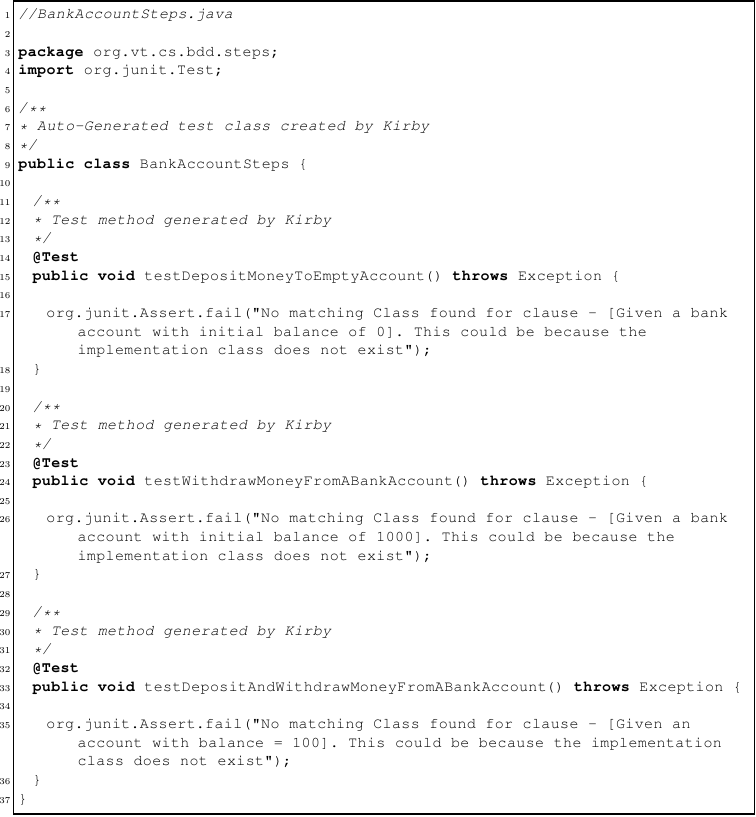
\includegraphics[width=0.7\linewidth]{Kirby_generated_test_class}
	\caption{Initially generated \textit{Kirby} tests}
	\label{fig:kirbygeneratedtestclass}
\end{figure}

The developer can now go ahead with the implementation of the class called BankAccount. Initially, we may only create the base class with the required constructor, in the Java project that is created.

\begin{figure}
	\centering
	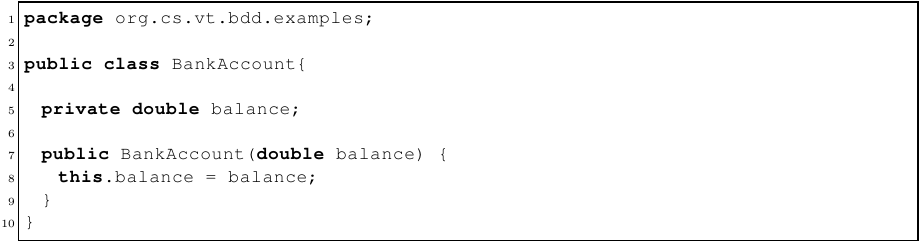
\includegraphics[width=0.7\linewidth]{BankAccount_class}
	\caption{The Initial BankAccount class}
	\label{fig:bankaccountclass}
\end{figure}

Now, if we run \textit{Kirby} on the story file again, it should recognize that a class called BankAccount has been created. Once it recognizes the class it should create code corresponding to the “Given” clause.

\begin{figure}
	\centering
	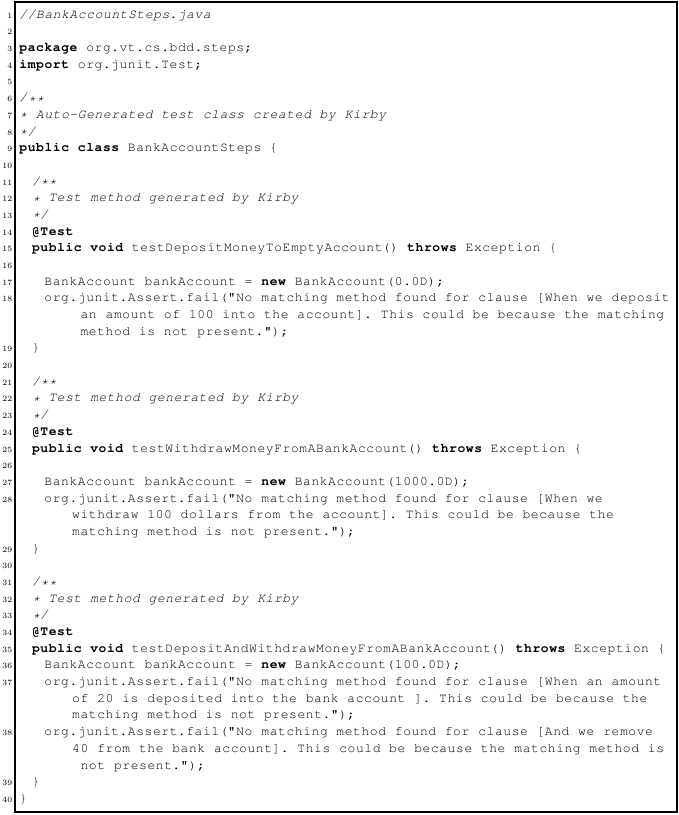
\includegraphics[width=0.7\linewidth]{Second_kirby_generated_test_class}
	\caption{\textit{Kirby} tests with BankAccount class incorporated}
	\label{fig:secondkirbygeneratedtestclass}
\end{figure}

In TDD style, we will add each method, then run the behavior, and further implement
the actual code. Once all those steps have been completed, the implementation for the BankAccount would update the glue code in the test cases in turn.

\begin{figure}
	\centering
	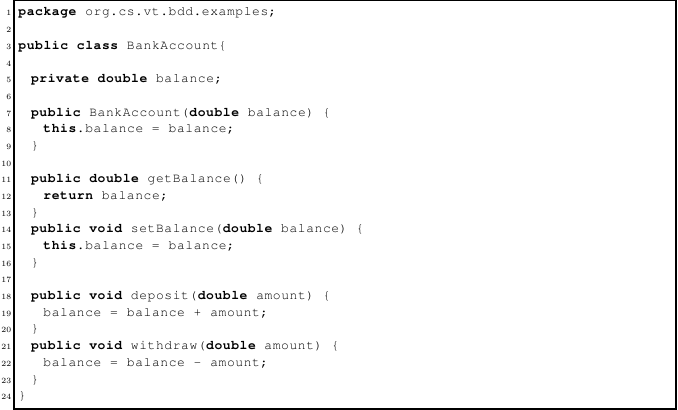
\includegraphics[width=0.7\linewidth]{BankAccount_class_implemented}
	\caption{BankAccount class with methods implemented}
	\label{fig:bankaccountclassimplemented}
\end{figure}

\begin{figure}
	\centering
	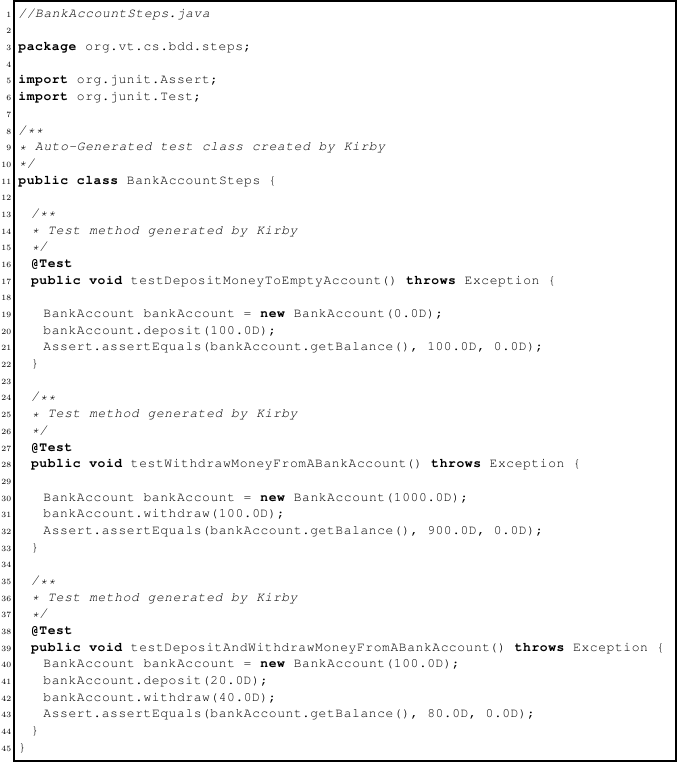
\includegraphics[width=0.7\linewidth]{Implemented_kirby_generated_test_class}
	\caption{\textit{Kirby} tests with BankAccount class methods incorporated}
	\label{fig:implementedkirbygeneratedtestclass}
\end{figure}

\subsection{User Interface of Kirby}
The UI is developed as a plug-in to Eclipse, which is a popular IDE. It helps in,
\begin{itemize}
	\item  Composing stories with the help of syntax highlighting for Gherkin based scenario descriptions.
	\item Auto-generating step definitions, which can be viewed and validated by the developer.
	\item Running auto-generated step definitions.
	\item  Viewing the results of the run, in a tabular form which indicates the success or failure of each scenario.
\end{itemize}

User stories can be written in any general text editor, and it should follow the convention of the Gherkin language. Also, the author has created a editor within the \textit{Kirby} UI which is capable of syntax highlighting various components of Gherkin language.

\begin{figure}
	\centering
	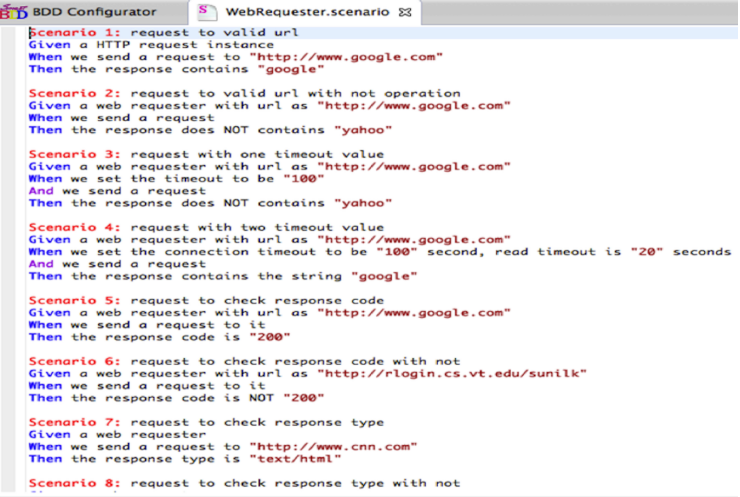
\includegraphics[width=0.7\linewidth]{Gherkin_editor}
	\caption{Gherkin editor in the UI}
	\label{fig:gherkineditor}
\end{figure}

Now that the stories have been created, the developer would want to be able to auto-generate the programmatic code, representing the scenario. In order to do this, he would use the main view of \textit{Kirby}. This view provides a convenient way of viewing the text in a story that the user has selected from the project. For a selected user story, the developer can click on a button, to auto-generate the corresponding step-definitions. He can view the auto-generated step definitions in the editor which is to the bottom right of the
main view, and validate it for correctness. 

\begin{figure}
	\centering
	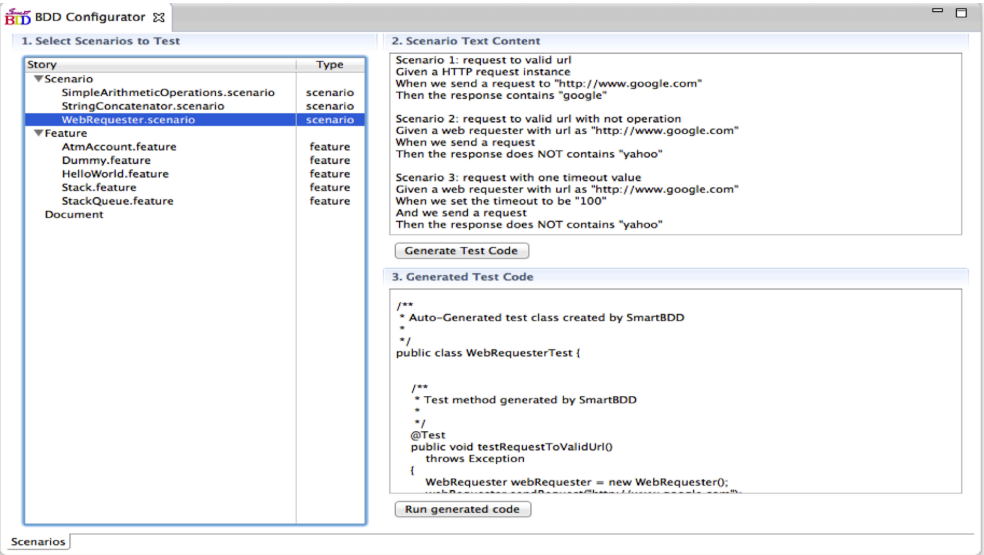
\includegraphics[width=0.7\linewidth]{Main_view_of_kirby}
	\caption{The main view of \textit{Kirby}}
	\label{fig:mainviewofkirby}
\end{figure}

Once the validation is done by the developer, he can click on a button to run the behavior as a JUnit test. Once the run is complete, the user is provided with a results page which indicates the status of the run. A tabular form of showing the results is followed, and for the selected behavior, a green color result indicates a success and a red color indicates a failure.

\begin{figure}
	\centering
	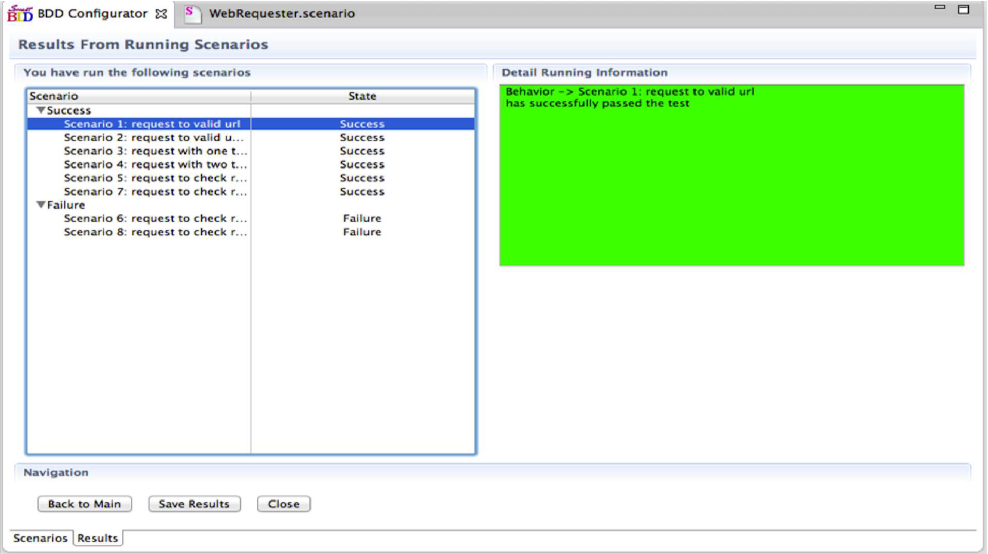
\includegraphics[width=0.7\linewidth]{Results_view_of_kirby}
	\caption{The results view of \textit{Kirby}}
	\label{fig:resultsviewofkirby}
\end{figure}

\subsection{Work flow of Kirby}
Developers alternate between creating or revising scenarios and writing implementation code. Since the implementation code is written with the scenario in mind, the author believes the language that is used in the code will naturally reflect the language of the scenario (with subtle variations). At any time, the scenarios can be executed directly on the implementation code by using \textit{Kirby}.

\begin{figure}
	\centering
	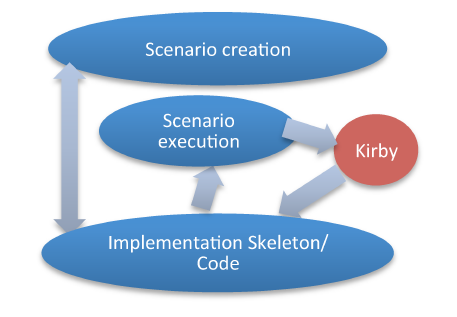
\includegraphics[width=0.7\linewidth]{System_workflow_kirby}
	\caption{System work flow of \textit{Kirby}}
	\label{fig:systemworkflowkirby}
\end{figure}

\subsection{Architecture of Kirby}
 As this system is code base aware, the author needed to develop a mechanism to map the natural language scenario descriptions onto code implementation that is being written alongside the scenarios. Kirby uses both the scenario descriptions and the co-developed software (complete code or stubs) as input when generating executable tests. It uses a Natural Language Augmentation Engine to process and augment the information in each clause of the scenario to understand its structure and semantics. At the same time, \textit{Kirby} also uses a reflection-based Class Information Extractor to obtain details about the classes and methods that have been written in the implementation. The Probabilistic Matcher determines the best matches between noun phrases and verb phrases in the behavioral description, and objects and methods available in the implementation. Once suitable matches have been found, the Code Generator synthesizes this information to produce JUnit-style tests.
 
\begin{figure}
	\centering
	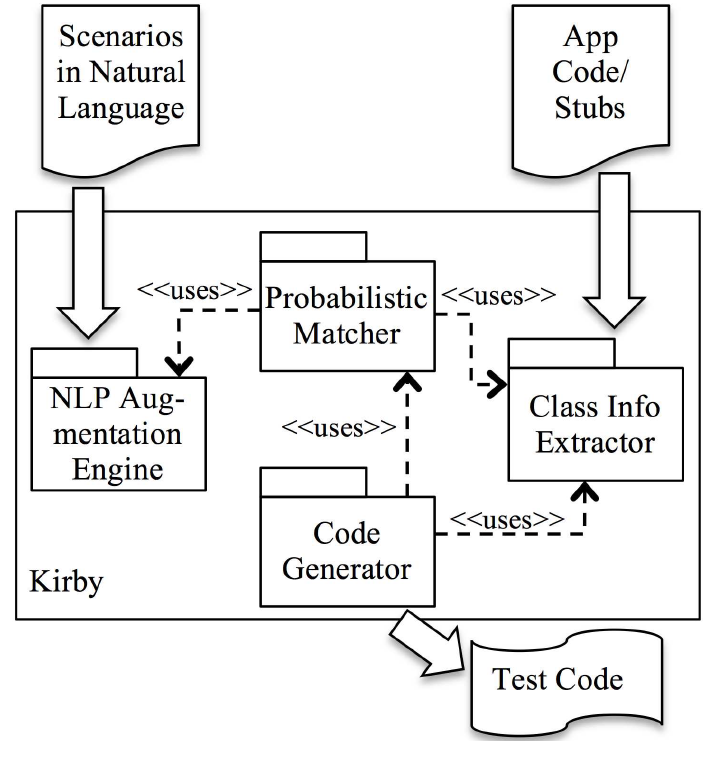
\includegraphics[width=0.7\linewidth]{Kirby_architecture}
	\caption{\textit{Kirby} High level Architecture}
	\label{fig:kirbyarchitecture}
\end{figure}

Since \textit{Kirby} supports Java with the generation of BDD glue code with the awareness of the code base, we focus more on supporting other languages.\newline

\section{Generative Adversarial Networks (GANs)}
\subsection{What is a GAN}

A GAN comprises of two neural network. One is used for model generation and the other is used for model validation. GANs are used in a variety of applications in the data science and machine learning domain. First introduced in the paper by I. J. Goodfellow, et at. titled "Generative Adversarial Nets" published in 2014. In it, they "propose a new framework for estimating generative models via an adversarial
process, in which we simultaneously train two models: a generative model G
that captures the data distribution, and a discriminative model D that estimates
the probability that a sample came from the training data rather than G." The adversarial modeling framework can be applied directly when the models are both multilayer perceptrons. To learn the generator’s distribution $p_{g}$ over data x, they define a prior on input noise variables $p_{z}(z)$ then represent a mapping to data space as $G(z; \theta_{g})$, where G is a differentiable function represented by a multilayer perceptron with parameters $\theta_{g}$. We also define a second multilayer perceptron $D(x; θ_{d})$ that outputs a single scalar. D(x) represents the probability that x came from the data rather than $p_{g}$. We train D to maximize the probability of assigning the correct label to both training examples and samples from G. We simultaneously train G to minimize $log(1-D(G(z)))$ \cite{b1}.

\subsection{Uses of GANs}

The scholarly work based on GANs include, using conditional generative adversarial nets for convolutional face generation wherein the authors, by varying the conditional information provided to an extended GAN, use the resulting generative model
to generate faces with specific attributes from nothing but random noise. An ideal training process for the above model would be
as follows: 
\begin{list}{*}{spacing}
	\item The generator outputs random RGB noise by default.
	\item The discriminator learns basic convolutional filters in
	order to distinguish between face images and random
	noise.
	\item The generator learns the correct bias (skin tone) and
	basic filters to confuse the discriminator.
	\item  The discriminator becomes more attuned to real facial
	features in order to distinguish between the simple
	“trick” images from the generator and real face images.
	Furthermore, the discriminator learns to use signals in
	the conditional data to look for particular triggers in
	the image.
\end{list} 

This process continues ad infinitum, until the discriminator is maximally confused. Since the discriminator outputs the probability that an input image was sampled from the training data, we would expect a “maximally confused” discriminator to consistently output a probability of 0.5 for inputs both from the training data and from the generator \cite{b2}. We can see that adversarial networks can be used to create useful cases of a target population and a model that would recognize the useful cases and filter them from a sample containing both useful and noise or unfit instances. Also, from this study we can see that even random noise can be used to generate useful instances.\newline
The authors T. Kim, M. Cha, H. Kim, J. Lee, and J. Kim have proposed a method based on generative adversarial networks that learns to discover relations between different domains (DiscoGAN). Inter domain relationships are very obvious to people, unlike it is for machines. For example, we recognize the relationship between an English sentence and its translated sentence in French.It is fair to consider and contemplate whether machines can also discriminate and also see the inter-relationships among various domains. The authors have addressed this in the form of a conditional image generation problem. In other words, authors tried to find a mapping function from one domain to the other can be thought as generating an image in one domain given another image in the other domain. The authors also note that this problem also brings an interesting challenge from a learning point of view as explicitly supervised data is seldom available and labeling can be labor intensive. Moreover, pairing images can become tricky if corresponding images are missing in one domain or there are multiple best candidates. So, the authors have resolved to automate the discovery of relations between two visual domains without any explicitly paired data \cite{b3}. From this study we can deduce that it is possible to discover the relationships between two domains using GANs and thus generate a GAN that would use inputs from one domain to generate instances in another domain. Thus, it is justifiable to assume that it is feasible to generate test cases, which are formed conforming to the rules of a programming language such as C++, Java, Python, etc. from use cases specified in natural language. In the final model, we shall use GANs to train for the generation of cohesive and compilable, runnable test cases, when the names of the classes and the methods, variables are discerned beforehand and fed into the GAN by the rest of our system.\newline

\section{Modern Software Development}
Modern software development involves much more than the simple writing of code. Test driven development was the first step in creating code that was more reliable, maintainable and consistent. With the recent popularity of agile methodology and push towards code quality, tests and test automation has become very important for development. Today, Test driven development has recently re-emerged as a critical enabling practice of the extreme programming software development methodology. L. Williams, E. M. Maximilien and M. Vouk ran a case study of this practice at IBM. In the process, a thorough suite of automated test cases was produced after UML design. In this case study, they found that the code developed using a test-driven development practice showed, during functional verification and regression tests, approximately 40\% fewer defects than a baseline prior product developed in a more traditional fashion. The productivity of the team was not impacted by the additional focus on producing automated test cases. This test suite aids in future enhancements and maintenance of this code. The case study and the results are discussed in detail in this study \cite{b4}. From the study we can see that TDD can improve the quality of work and also can do so without impeding on the normal software development process. The current trend in software development are highly geared towards delivering quality software to clients, as quickly as possible. New methodologies such as Agile software development are being adopted in order to replace the old development methodologies such as waterfall. To accommodate this high quality and fast delivery process, it is imperative that the code is properly tested for the intended functionalities.\newline
Modern development definitely calls for TDD, but it is not sufficient. The test cases can be readable and understandable for the developer, but apart from the developer, other stakeholders within the project such as business analysts and the client. So, the next innovation within the software development testing was to change the way that the tests are written and used.\newline
Now the move is towards the automation of tests and writing code that is much more comprehensible. Now, manual testing is discouraged and automated test writing is encouraged. The availability of free and open source tools for test automation such as Jenkins speaks volumes about the importance of test automation. Automated test cases allows for more efficiency and can immediately notify the developer in the case that the code is broken. In the case that there are manual tests instead of automated tests, the developer has to run the tests manually and see if code has been broken. This is a problem if there are too many tests to be run manually. The move now is also towards writing tests based on the client requirements. This way  the developers can make sure that the client requirements are aligned with the actual development process.\newline
From manual testing, we have now moved onto TDD and subsequently, to BDD. In BDD, we have a practice that brings all stakeholders of a SE project together like never before in the history of SE practices. Helping developers to embrace this practice will be to the benefit of their organizations and the stakeholders within their organizations and also, most important of all, the developers themselves.\newline

\section{Test Driven Development: Prelude To BDD}
In \textit{A Comparative Case Study on the Impact of Test-Driven Development on Program Design and Test Coverage}, it is mentioned that "Test-driven development (TDD) is a programming technique in which the tests are written prior to the source code. It is proposed that TDD is one of the most fundamental practices enabling the development of software in an agile and iterative manner. Both the literature and practice suggest that TDD practice yields several benefits. Essentially, it is claimed that TDD leads to an improved software design, which has a dramatic impact on the maintainability and further development of the system." \cite{b6} TDD in actuality is a development technique rather than a testing technique \cite{b7}. The tests are iteratively added throughout the implementation and when the tests pass, the code is refactored to improve its internal structure. This incremental cycle is repeated until all the functionality is implemented \cite{b8}. The idea of TDD was popularized by Beck \cite{b9} in the Extreme Programming (XP) method. Therefore, although TDD seems to have just recently emerged, it has existed for decades; an early reference to the use of TDD features in the NASA Project Mercury in the 1960s \cite{b10}. 
Both the literature and practice indicate that the use of TDD yields several benefits. Among others, TDD leads to improved test coverage \cite{b8} and simplifies the design by producing loosely coupled and highly cohesive systems \cite{b11}. TDD also enables the implementation scope to be more explicit. As a positive side effect, TDD may lead to enhanced job satisfaction and confidence \cite{b11}. Also, larger teams of developers can work on the same code base because of the more frequent integration \cite{b7}.  But, TDD has also been criticized for not compensating the lack of up-front design and not being very suitable for systems such as security software or multi-threaded applications, since it cannot mechanically demonstrate that their goals have been met \cite{b12}. It is also claimed that rapid changes may cause expensive breakage in tests and that the lack of application or testing skills may produce inadequate test coverage \cite{b13}. However, the scientific empirical evidence behind these claims is currently scattered and disorganized, and thus it is difficult to draw meaningful conclusions. Moreover, studies addressing the impact of TDD on program design are currently very rare \cite{b6}.
The work by Maria Siniaalto and Pekka Abrahamsson states that, The results partially contradict the current literature as the empirical evidence shows that TDD does not improve the program design as expected. In particular, TDD does not necessarily produce highly cohesive systems when employed by non-professional developers. However, TDD appears to result in significantly better test coverage than the iterative test-last development. The findings are based on three software development projects, two of which used iterative test-last development and one utilized TDD \cite{b6}.\newline
B. George and L. Williams et al. have stated that, "..we find the definition of TDD as, before writing implementation code, the developer writes automated unit test cases for the new functionality they are about to implement. After writing test cases that generally will not even compile, the developers write implementation code to pass these test cases. The developer writes a few test cases, implements the code, writes a few test cases, implements the code, and so on. The work is kept within the developer’s intellectual control because he or she is continuously making small design and implementation decisions and increasing functionality at a relatively consistent rate. A new functionality is not considered properly implemented unless these new unit test cases and every other unit test cases ever written for the code base run properly." \cite{c1} Maria Siniaalto et al. has compiled results from empirical studies conducted on TDD to evaluate the value of TDD as an engineering practice. In this study, they have looked at the studies of Bhat and Nagappan. They present the results of two industrial case studies conducted at Microsoft. They compared the impacts of TDD and non-TDD development processes on quality and overall development time. Their results show that the quality of the code developed using TDD increased $2.6-4.2$ times when compared to non-TDD developed code. Alternatively, the project managers estimated that TDD increased the overall development time by $15-35$ \%. The block coverage was $79-88$ \% at unit test level in projects employing TDD. They also noticed that the tests serve as auto documentation when the code was maintained or used \cite{c2}.\newline

\section{Behaviour Driven Development (BDD)}
\subsection{What is BDD?}
Behaviour Driven Development is a relatively new branch of development wherein the client requirements are used as the baseline for generating the test cases. This is a solution to the problems we have introduced during the last section. The test cases are based completely on the requirements provided by the client. So the development process will be completely aligned with the client requirements. This results in tests that test for the end-user use cases rather than much more abstract conditions.\newline
The business analysts can note down the client requirements in the following manner, highlighting their requirements so that it would be possible to discern the conditions required for user acceptance.
\begin{itemize}
	\item GIVEN: The client's initial state.
	\item WHEN: The change that takes place, it can be a change made by the client or some other event that takes place which is not controlled by the client.
	\item THEN: The expected behaviour when the change occurs.
\end{itemize}
We can translate such requirements directly into test cases. The methodology to be followed in such a scenario is as follows;
\begin{itemize}
	\item GIVEN: The starting condition. Initial conditions that we take are available at the start of the test.
	\item WHEN: The change that happens or is expected to happen. This is a disruptive event that will cause the event that will setup the expected response.
	\item THEN: The test scenario. The response that we are looking for after the disruption condition.
\end{itemize}

Following Fig. 11 is an example from the cucumber BDD test case.

\begin{figure}
	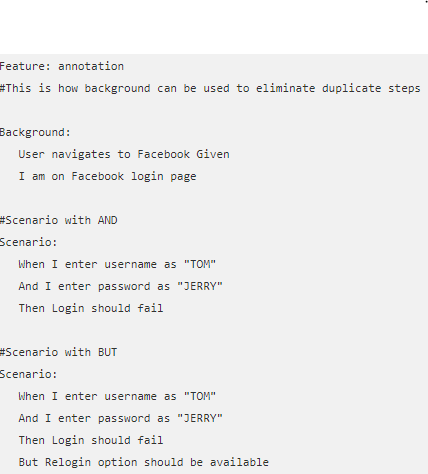
\includegraphics[width=\linewidth]{cucumber_figure.png}
	\caption{Example of Cucumber Test Execution}
	\label{fig1}
\end{figure}

Dan North invented BDD to transform TDD into a more efficient software development process \cite{d2}. The main goal of BDD is to get executable and well-defined specifications of software \cite{d2}. According to Dan North, the definition of BDD
is: “A second-generation, outside-in, pull-based, multiple-stakeholder, multiple-scale, high-automation, agile methodology” \cite{d3}. In other words, BDD combines general
techniques and principles of TDD with ideas from domain driven design and object-oriented analysis and design. This combination is done in order to provide software development and management teams with shared tools and a shared process to collaborate on a software development \cite{d1}. Following tables are taken from "A Literature Review of Behavior Driven Development using Grounded Theory" by Egbreghts et al. 2018 \cite{d1}.\newline

\begin{tabular}{|c|p{6cm}|}
	\hline 
	Phases & TDD \\ 
	\hline 
	1 & Write a test \\ 
	\hline 
	2 & Run the test and check
	if it fails \\ 
	\hline 
	3 & Write a code sufficient
	for the test to pass \\ 
	\hline 
	4 & Run the test and check
	if it passes \\ 
	\hline 
	5 & Refactor the code \\ 
	\hline 
\end{tabular} 

\begin{tabular}{|c|p{6cm}|}
	\hline 
	Phases & BDD \\ 
	\hline 
	1 & Write a test scenario \\ 
	\hline 
	2 & Execute the scenario and
	check if it fails \\ 
	\hline 
	3 & Write a code sufficient to
	implement the expected
	behavior \\ 
	\hline 
	4 & Execute the scenario and
	check if it passes \\ 
	\hline 
	5 & Refactor the code \\ 
	\hline 
\end{tabular} 

According to two papers, ubiquitous language is the fundamental core of BDD \cite{d4, d5}. the meaning of ubiquitous language is derived from the book written by Eric Evans named Domain-driven design (DDD). According to Evans, ubiquitous language is a familiar
language, structured around the domain model, shared by both business and IT stakeholders to communicate the tasks connected to the software development \cite{d6}. The terms in the
language are derived from the natural way of speaking, like whenever the clients try to explain to developers what for software they want, they use easy phrases, such as “when I do that, then this should happen” \cite{d7}.\newline
According to North, there are two predetermined specifications that are essential to BDD which are user stories and scenarios \cite{d2}. First of all, a scenario is composed of several step definitions. A step is an abstraction that represents one of the elements in a scenario, which are contexts, events, and actions. The meaning of them is: in a particular case of a user story A, when event B happens, the answer to the system should be C. One step is mapped to one test method \cite{d4}. Namely, each scenario composes of one test case, in which each sentence is referred to as a step \cite{d8}. Secondly, user stories are written to identify features and a feature is used to group a set of scenarios. BDD offers to users a template for both scenario and user story description \cite{d1}. The goal of these requirements are to capture the needs of the customer, to map them into the code, and to ensure that the developers are developing the right software \cite{d9}. This in turn helps to guide the developers in knowing what to test as well as understanding what features are required to be implemented to pass tests and to write tests that are understood by all stakeholders \cite{d10}.\newline

\begin{figure}
	\centering
	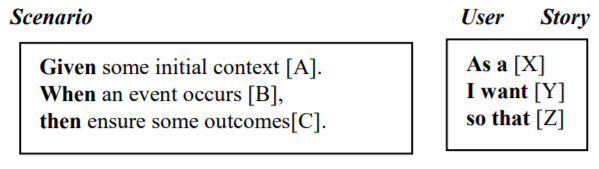
\includegraphics[width=0.7\linewidth]{scenario_user_story}
	\caption{Scenario and User/Story description}
	\label{fig:scenariouserstory}
\end{figure}


\section{Generation of tests with from text descriptions}
\subsection{Justification}
Generation of test cases is akin to generating images using text, in the sense that what we are attempting to do is generate a representation of a highly structured text description, in another domain. Han Zhang et al. have done a study wherein they synthesize high-quality images from text descriptions as samples generated by existing text-to-image approaches can roughly reflect the meaning of the given descriptions, but they fail to contain necessary details and vivid object parts. The authors have had much success in generating images which fit the plain text descriptions of them, as specified \cite{b5}. Our case is similar in that we are using a user specified plain text to generate compilable and working test code. The success of the previous studies encourage us in that we can achieve our task of generating test cases directly from the plain text descriptions of the functionality.

\begin{figure}
	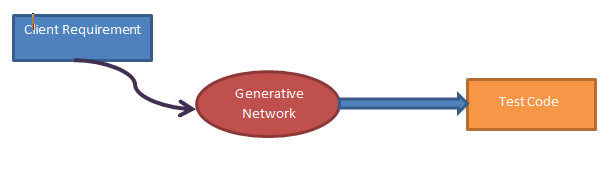
\includegraphics[width=\linewidth]{Generative_network.png}
	\caption{The functionality of the generative network}
	\label{fig2}
\end{figure}

\subsection{Initial Proposed Model}
This section describes the initial plan/proposal for the implementation of the test code generation system I came up with. Afterwards, it went through many refinements but some of the basics used here, remained.

\subsubsection{The Generative Network}
As displayed by the Fig. 13, the task of the generative network is to look at the client requirement of a functionality, here we introduce the constraint that it must follow a certain format. The format being the language we use when specifying a requirement when we write down a BDD test scenario, Gherkin. That is, it must follow the basic structure of,

\begin{itemize}
	\item Scenario
	\item GIVEN
	\item WHEN
	\item THEN
\end{itemize}

\begin{figure}
	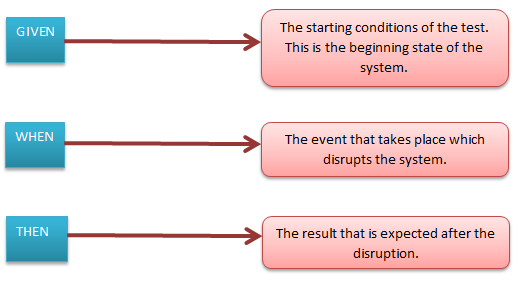
\includegraphics[width=\linewidth]{Given_when_then.png}
	\caption{BDD Test case structuring}
	\label{fig3}
\end{figure}

based on the descriptions, the generative network will be able to infer class names and their members, methods and their signatures. Initially, we thought of feeding the client requirements directly to the generative network but afterwards, thought of feeding processed input to it, in order to make the training process easier.

\subsubsection{Validation Network}
There are two types of possible validations for our case. These are, checking consistency with the written test case and checking the consistency with the programming language. Here, we have a network that checks the code compilation validity and another network that checks the validity of the generated code against the programming language specification.

\begin{figure}
	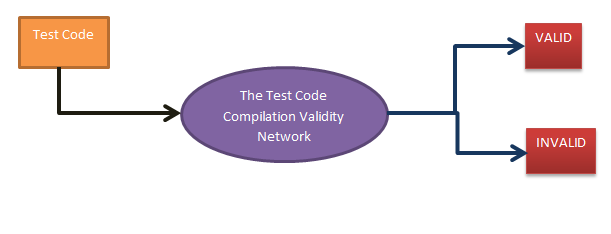
\includegraphics[width=\linewidth]{Compilation_validity.png}
	\caption{Compilation validity checking network}
	\label{fig4}
\end{figure}

We can also have a network that can check the validity against the test case as well. But for this project we shall only concentrate on the prior network. We shall leave the possibility of adding a check for consistency with the test specification as future work. The validation networks, as specified here, are suggestions based on the functionality and can also be unified if necessary.

\subsection{Types of networks usable}

\subsubsection{Recurrent Neural Networks}
\subsubsection{On End-to-End Program Generation from User Intention by Deep Neural Networks}
Lili Mou, Rui Men, Ge Li, Lu Zhang, Zhi Jin et al. 2015, have put forward this study. This paper envisions an end-to-end program generation scenario
using recurrent neural networks (RNNs): Users can express their intention in natural language; an RNN then automatically generates corresponding code in a character-by-character fashion. The authors demonstrate its feasibility through a case study and empirical analysis. For end-to-end program generation, they prefer the RNNs, which are suitable for modeling time-series data (e.g., a sequence of characters) by its iterative nature. An RNN typically keeps one or a few hidden layers, changing over each (discrete) time step according to input data.\newline
Theoretical analysis shows that recurrent neural networks are equivalent to Turing machines \cite{a6}. However, training RNNs in early years was difficult because of the gradient blowup or vanishing problem \cite{a7}. Long short term memory
(LSTM) units \cite{a8}, or gated units \cite{a9} are designed to balance
between retaining the previous state and memorizing new information at the current time step, making RNNs much easier to train.\newline
On this basis, Sutskever et al. design an RNN model for sequence to sequence generation \cite{a10}. The idea is to first read an input sequence, ended with a special symbol, $<eos>$ (end of sequence). For output, the RNN applies a softmax layer at each time step, predicting the probability that each symbol may occur at the current step; the symbol with the highest probability is chosen, and fed to the network as input at the next time step. This process is done iteratively until the special symbol, $<eos>$, is generated by the network.\newline
Such RNN architecture can be applied to sequences of different granularities, e.g., word-level, sub-word level, etc. In particular, character-level RNN generative models have unexpectedly achieved remarkable and somewhat amazing performance. Successful applications include generating texts, music, or even Linux-like C code. \cite{a11} Empirical studies show that RNNs are particularly good at modeling syntax aspects, e.g., parenthesis pairing, indentation, etc. \cite{a12} It works much like a push-down automata, but seems less capable of capturing semantics—the Linux-like code generated, for example, is plausible, but cannot be compiled and lacks coherence in functionality.
The authors are therefore curious whether RNNs can generate executable, functionally coherent source code, which is an essence to benefit real-world software engineering tasks.
To accomplish this goal, the authors leverage a dataset from a pedagogical
programming online judge (OJ) system,(http://programming.grids.cn) intended for the undergraduate course, Introduction to Computing. The OJ system comprises different programming problems. Students submit their source code to a specific problem, and the OJ system judges its validity automatically (via running).

\begin{figure}
	\centering
	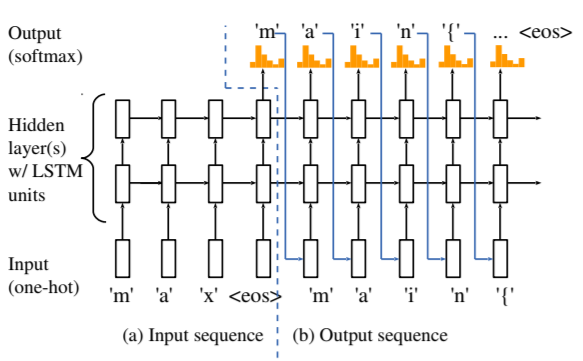
\includegraphics[width=0.7\linewidth]{sequence_to_sequence_recurrent_neural}
	\caption{Sequence to sequence recurrent neural network}
	\label{fig:sequencetosequencerecurrentneural}
\end{figure}

\begin{figure}
	\centering
	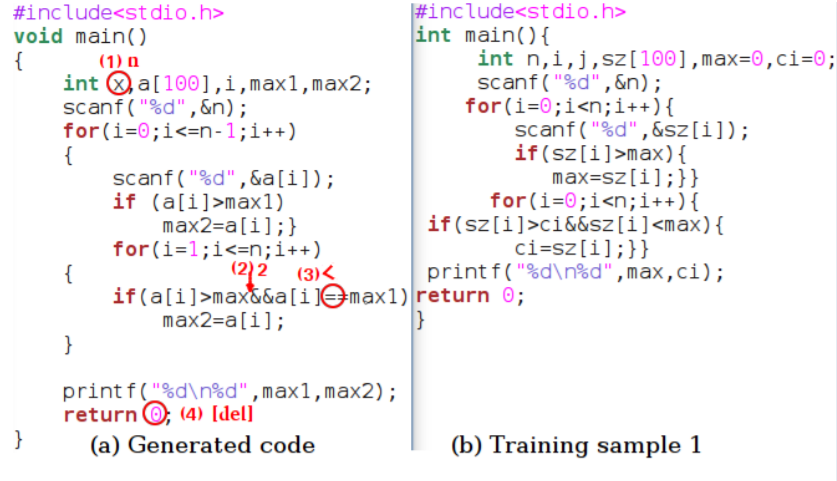
\includegraphics[width=0.7\linewidth]{Training_and_generated_code}
	\caption{Training and Generated Code Samples}
	\label{fig:trainingandgeneratedcode}
\end{figure}

\begin{figure}
	\centering
	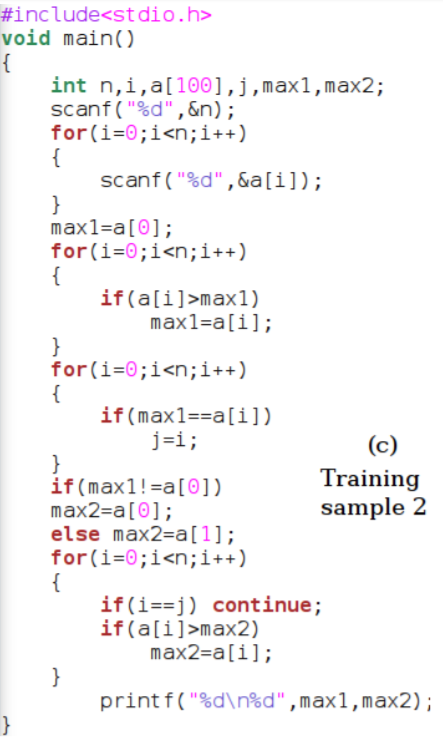
\includegraphics[width=0.7\linewidth]{Second_training_sample}
	\caption{Second training example}
	\label{fig:secondtrainingsample}
\end{figure}

The authors notice that programs corresponding to a specific problem have exactly the same functionality, which makes the dataset particularly suitable, as a first trial, for training neural networks to generate functionally coherent programs.
The authors have fed the network with 4 different programing problems, each containing more than 500 different source code samples. After preprocessing, a program was preceded by a brief comment, e.g., “find the maximum and second maximum numbers,” serving as the input sequence (Fig. 16a). What follows is a program that solves the particular problem, serving as the output sequence (Fig. 16b). Figures 17b and 18 further illustrate two training samples of the aforementioned programming problem.
The results of the authors' work is as follows, Figure 17a is a sample code generated by RNN. Through a quick analysis, authors find that the code is almost executable: with a little post-correction of 4 characters among around 280, the program is compilable and functionally correct. Authors would answer a very fundamental question: Is RNN generating code by simply memorizing a particular training sample? If this were the case, RNN would just work in a copy-and-paste fashion, which degrades the problem to a trivial case.
By examining the training data, authors observe that there does not exist a same program in the training set, which rules out the possibility that RNN works by exact memorizing. Authors further use ccfinder \cite{a4} to detect most similar code in the training set. Two are shown in Figure 17, and the results are particularly interesting. Authors provide their explanation regarding several aspects of a program as follows.

\begin{itemize}
	\item \textbf{Structure:} Figure 17b shows the most similar code in
	structure. The generated code implements the same
	algorithm—scanning the array twice to find the maximum
	and second maximum numbers respectively. Notice,
	however, the two structures (abstract syntax trees,
	say) are not exactly the same as there are differences in
	variable definitions. A more interesting detail is that
	RNN has recognized $“i<n”$ and $“i<=n-1”$ are equivalent
	in the for loop, and that it does not follow exactly the
	sample code (b) in the training set but remains correct.
	\item \textbf{Variable IDs:} The training sample with the most
	similar variable IDs is shown in Figure 18. Our generated
	code uses the same ID, a, for the array, and \textit{max1,
	max2} to cache the two wanted numbers; but later, the
	structure diverges. Nevertheless, our network is aware
	of the variable IDs it has generated, and remains coherent
	until the very end of the program.
	\item \textbf{Style:} Authors find no particular training samples having
	the same code style in terms of indents, line feeds, etc.
	It makes much sense because the training programs are written by junior programmers, who may not follow standard style convention, and thus the network has no idea about the “right” style. However, as all training
	samples are “correct” programs, our network has little difficulty in learning the syntax of C programs as the generated code can almost be compiled.
\end{itemize}

Through the above analysis, authors, and we, gain a basic idea on how RNN is able to generate programs. The RNN first recognizes the brief comment, “find the maximum and second maximum numbers,” which precedes the code as input. The authors would like to point out that, in this experiment, the RNN does not understand the meaning of this sentence; but via reading the brief comment, the RNN switches its hidden states to generate code of the functionality in need. For each functionality, RNN is aware of different aspects of a possible program, including structures, IDs, etc. When generating, it chooses the most likely character conditioned on the previous characters, also conditioned on the input. In particular, the RNN does have the ability to mix different structures and IDs but remain (almost) coherent.\newline
Under the Prospectives and Road map section, the authors have described their work as simple and preliminary, and that their case study and analysis provide great insights into the end-to-end program generation with deep neural networks. They have considered several scenarios where deep learning can benefit real-world SE
practice, which are also research topics in long-term studies. They are,

\begin{itemize}
	\item \textbf{Understanding changeable user intention:} The current case study shows RNN’s ability of recognizing certain intentions and generating corresponding code. In the general SE practices, however, there are oftentimes requirements that are subject to change. A solution is to train a parametric code generator with arguments (e.g., file names, protocols) implicitly
	expressed using natural language. To tackle
	a more challenging prospective, the authors suggest to first train
	a network to generate different “primitive” code snippets,
	and then “glue” them together. For instance, if a network has learned to write code of finding the maximum number, and also of finding the minimum
	number, then it shall be possible to generate these two
	snippets subsequently if it reads an instruction “find
	the maximum and minimum numbers.”
	\item \textbf{Incorporating multiple sources of user intention.} When
	developing software, programmers usually find their code dependent to context (e.g., previously defined variables, existing API call sequences) in addition to the functionality in need. In such scenarios, the authors suggest that we might train a network to fill missing blocks of code. While authors admit that code completion in general could hardly
	make any sense, we think this problem is mostly realistic in some task-specific scenarios. For example, a typical way of reading a txt file in Java involves creating FileReader, BufferedReader, reading lines in
	the file, closing the file, and also catching exceptions.
	Such standard pipelines might be generated automatically
	by neural networks, provided context code.
\end{itemize}

The authors note that the most important questions in the SE community are defining user’s intention and providing datasets for training. The open questions within this study's context are,
\begin{itemize}
	\item How to specify the functionality that we want to generate? 
	\item How to specify the arguments of a function? 
	\item How to collect the dataset which is not only large and informative
	enough for training, but also clean enough for not including
	too much noise?
\end{itemize}

Also, the authors concede that using RNNs to generate programs differs
significantly from writing programs by humans. It appears that it is unrealistic, currently, to train any learning machine, including deep neural networks, to fully understand either natural languages or programming languages. However, supported
by existing evidence in the literature and the case study in
this paper, they deem end-to-end program generation shall be possible in the future.\newline
When looking at this study, we can see great similarities between what the authors tried to achieve and what we are designing. A major difference although is that our text descriptions (written in Gherkin) have less variability than the usual specification of a functionality in plain text is. So it is plausible that our case where trying to generate test cases from Gherkin specifications is much simpler. But it is also worth noting that even then, there has been very little work performed in the area of test case generation using neural networks.

\subsubsection{Source Code Generation from User Intention by Using Recurrent Neural Networks}
In his 10th March 2017 blogpost, Albertus Kelvin has described a research with the intention to "develop an automatic programming system that could receive problem statement written in natural language and then generate the relevant source code...In addition, the system will use RNNs to achieve the goal."\cite{a3} In this article, the author has discussed the implementation of the "On End-to-End Program Generation from User Intention by Deep Neural Networks" by Lili Mou, Rui Men, Ge Li, Lu Zhang, Zhi Jin et al. 2015, which was discussed in the previous section.\cite{a3}\newline
When considering the training procedure for this RNN is as follows,
\begin{enumerate}
	\item Preprocessing the problem statement to remove noise.
	\item Primary context which is described in a brief statement. 
	This context tells the machine what the user intention is. Each of the characters of the context statement will be processed in the input layer as the input sequence.
	\item The learning process is supervised. So the corresponding source code is provided as the output sequence. After the last character of input sequence, the model will start to generate the output sequence by using the softmax layer, as described before.
\end{enumerate}

\begin{figure}
	\centering
	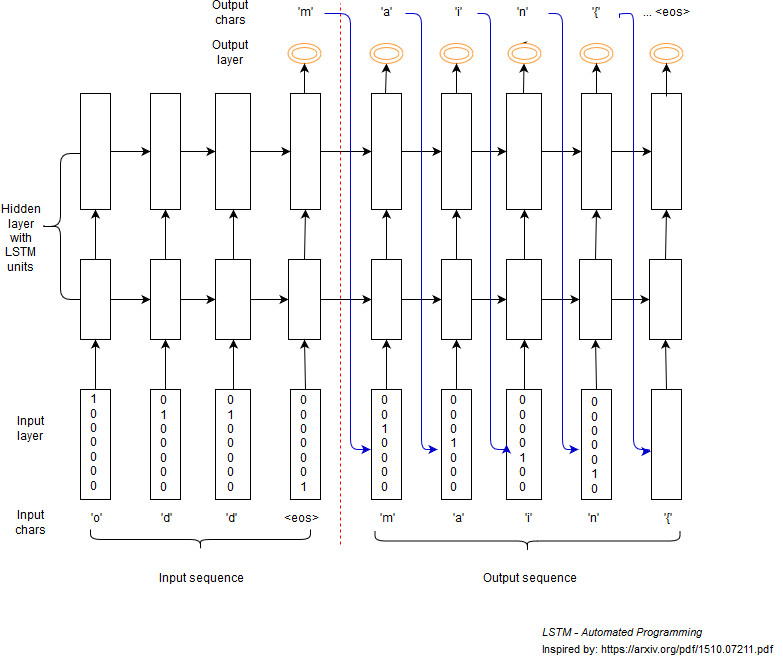
\includegraphics[width=0.7\linewidth]{RNN_model}
	\caption[Sequence to sequence RNN]{Sequence to sequence RNN by Albertus Kelvin et al. 2017}
	\label{fig6}
\end{figure}

The evaluation of the model is as follows, the author uses ccfinder \cite{a4} to find the most similar code in the training data. The general scenario is that the author will compare the generated source code with all the codes that were found by ccfinder. There are several aspects of the generated code that will be considered in the evaluation stage, such as structure, variable IDs, and style. For the structure aspect, the author checks whether the generated code implements the same algorithm. For the variable IDs aspect, author checks whether the generated code has different names for its variables but still retains the correct algorithm. For the last aspect, author checks whether the generated code provides different code style in terms of indentation, line feeds, and so on.\newline
The blog post however does not provide a view to the results of the activity. It simply outlines the methodology and the theory.

\subsubsection{The Unreasonable Effectiveness of Recurrent Neural Networks}
In his blog post "The Unreasonable Effectiveness of Recurrent Neural Networks", Andrej Karpathy discusses why recurrent neural networks are more successful than the other types of neural networks such as convolutional and vanilla networks. He mentions that, a glaring limitation of Vanilla Neural Networks (and also Convolutional Networks) is that their API is too constrained, that, they accept a fixed-sized vector as input (e.g. an image) and produce a fixed-sized vector as output (e.g. probabilities of different classes). Not only that, These models perform this mapping using a fixed amount of computational steps (e.g. the number of layers in the model). The core reason that recurrent nets are more exciting is that they allow us to operate over sequences of vectors: Sequences in the input, the output, or in the most general case both \cite{a11}.

\begin{figure}
	\centering
	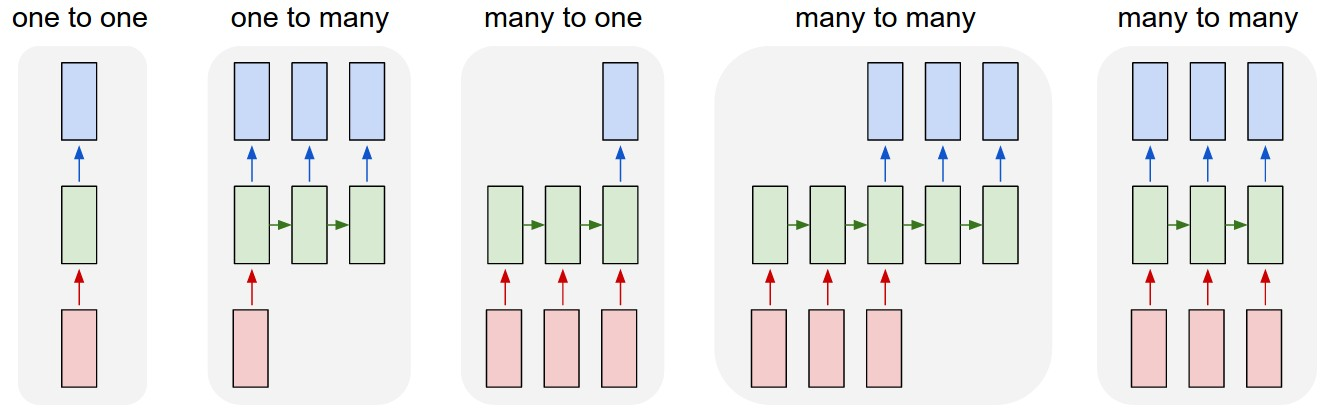
\includegraphics[width=0.7\linewidth]{recurrent_neural_network}
	\caption{Recurrent neural network architectures}
	\label{fig:recurrentneuralnetwork}
\end{figure}

In the figure displaying the recurrent neural network architectures, which is taken from the same blog post, each rectangle is a vector and arrows represent functions such as matrix multiplication. Input vectors are in red, output vectors are in blue and green vectors hold the RNN's state. From left to right, 
\begin{enumerate}
	\item Vanilla mode of processing without RNN, from fixed-sized input to fixed-sized output (e.g. image classification).
	\item Sequence output (e.g. image captioning takes an image and outputs a sentence of words).
	\item Sequence input (e.g. sentiment analysis where a given sentence is classified as expressing positive or negative sentiment).
	\item Sequence input and sequence output (e.g. Machine Translation: an RNN reads a sentence in English and then outputs a sentence in French).
	\item Synced sequence input and output (e.g. video classification where we wish to label each frame of the video).
\end{enumerate}
Notice that in every case are no pre-specified constraints on the lengths sequences because the recurrent transformation (green) is fixed and can be applied as many times as we like. The sequence operation is much more powerful compared to fixed networks that are restricted at design by a fixed number of computational steps, and hence also much more appealing for those of us who aspire to build more intelligent systems. Moreover, RNNs combine the input vector with their state vector with a fixed (but learned) function to produce a new state vector. This can in programming terms be interpreted as running a fixed program with certain inputs and some internal variables. Viewed this way, RNNs essentially describe programs. In fact, it is known that RNNs are Turing-Complete in the sense that they can to simulate arbitrary programs (with proper weights). It is possible to think that having sequences as inputs or outputs could be relatively rare, but an important point to realize is that even if inputs/outputs are fixed vectors, it is still possible to use this powerful formalism to process them in a sequential manner \cite{a11}.\newline

In the same blog post, under the Linux Source Code section, the author mentions that he wanted to push structured data to its limit, so he decided to use all the source and header files found in the Linux repo on Github, concatenated all of them in a single giant file (474MB of C code). These models have about 10 million parameters and the result of the code generation is a code which is not necessarily compilable but is consistent with the Linux code base \cite{a11}.

\begin{figure}
	\centering
	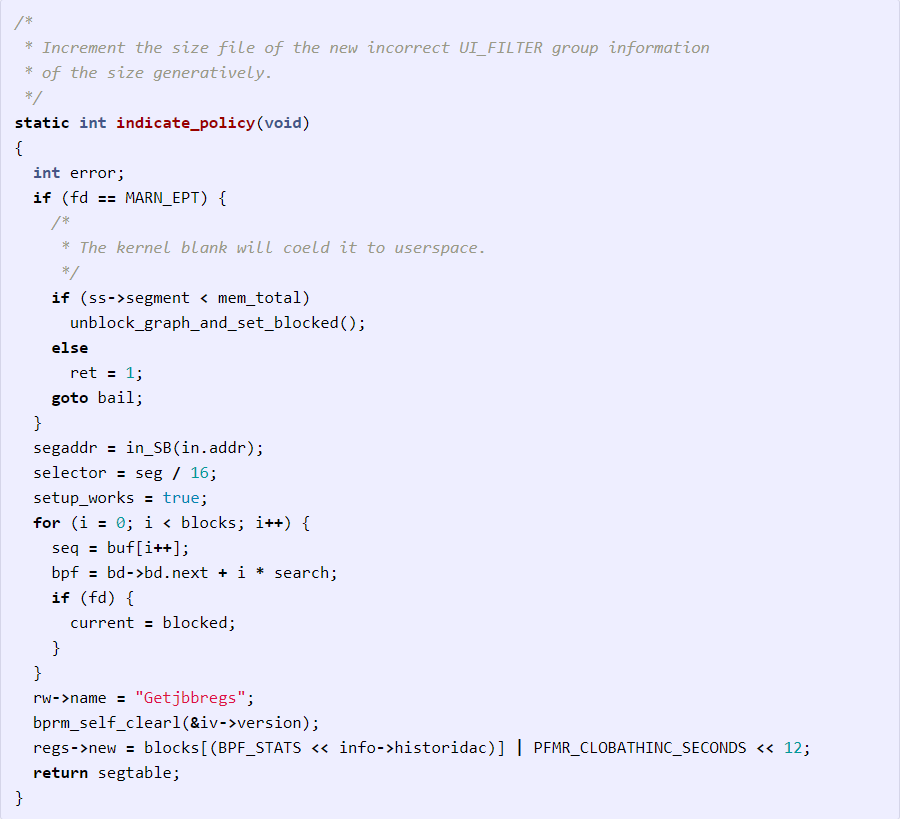
\includegraphics[width=0.7\linewidth]{Karpathy_gen_code}
	\caption{Code generated by A. Karpathy's RNN based on the Linux Code Base}
	\label{fig:karpathygencode}
\end{figure}


\section{Methodology}
The final design of the system is discussed in this section. We intend to support multiple programming languages in this approach. The model has been expanded and elaborated upon. Now, there are 6 major modules in the system. They are:

\begin{figure}
	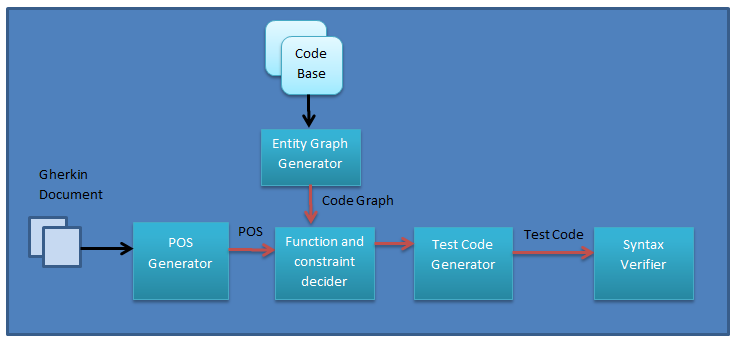
\includegraphics[width=\linewidth]{Complete_high_level_modules.png}
	\caption{Complete high-level model}
	\label{fig14}
\end{figure}

\begin{enumerate}
	\item \textbf{The Token Extractor:}
	Breaks down the Gherkin test case to useful text tags. This is a NLP module. Does not depend on the programming language selection.
	\item \textbf{Entity Graph generator:}
	Scans the whole code base and breaks them down into a useful format that is understood by our system. (Actually, by the third module)
	\item \textbf{Language Decider:}
	Looks at the code samples and decides the programming language and then loads the relevant libraries for the other modules.
	\item \textbf{Entity Relationship Extractor:}
	Looks at the tags and the code representation given to the module and decides the text-to-code mappings. This has NLP elements as well. Depends on the programming language selection.
	\item \textbf{User Interface:}
	User Interface is provided to the user in order for the user to interact with the system and to disambiguate or clarify system's code generation decisions with the user.
	\item \textbf{Test Code generator:}
	Based on the selections and decisions, create the test case. Depends on the programming language selection. This is the generative section of the GAN.
	
\end{enumerate}

Let's examine the modules in detail in the next section.

\subsection{The Token Extractor}
This module is capable of reading Gherkin files. It will process a single file at a time. The target of this module will be to extract the necessary tags from the file. Here, we will be considering the types of data that is contained within each of the cases in BDD. Let us examine the types of data that can be extracted from each of the Gherkin keywords.

\begin{itemize}
	\item \textbf{Feature:}
	Feature is the first keyword that we encounter when processing BDD specs. It is the topic under which the test cases are organized. Following the feature, there are lines describing the overall feature, which is usually used as comments. but we can use it for the deduction of functionality, but we must give it less emphasis as it is used as comments in most cases. It may be possible to discover functional and member bindings within the class through the feature descriptions.
	\item \textbf{Example/Scenario:}  
	This is the specification of a scenario, i.e. a BDD test case. From this section we can extract the name for the test case. Following this section are all of the step definitions, which make up the test case scenario. These will be the major source for the extraction of relationships.
	\item \textbf{Steps:}
	These contain the keywords, Given, When, Then, And, But. Given provides the initial setup conditions. The initial step should describe how the initial setup is done with enough clarity to unambiguously decide the classes and methods to call. We have to identify and pass the possible class and method and variable names and their relationship indicating words forward through the system. When represents a disruption within the system, hence it would be a specific input, either it is a certain signal or an object that is passed to the SUT. When is concerned about the output of the SUT. So to facilitate the recognition of these entities, we should pass the text values that would allow for the successful identification of the values for these entities and the ways in which we can capture these values.
	\item \textbf{Background:}
	Background is similar to a given statement that spans throughout multiple test cases. So we can treat it similar to the way we would treat a "Given" statement.
	\item \textbf{Scenario Outline:}
	The Scenario Outline keyword can be used to run the same Scenario multiple times, with different combinations of values. \ref{fig13} demonstrates an instance where a scenario outline is used \cite{a1}. Here, we can see the test case being parameterized and given multiple values for the input, signal and output values. Our system should be able to identify the parameters and the values associated with them, and pass them forward.
	\item \textbf{Doc Strings:}
	The doc string is passed as the last argument of a step definition when it is specified. We have to treat the string as an immutable value and pass it forward through the system.
	\begin{figure}
		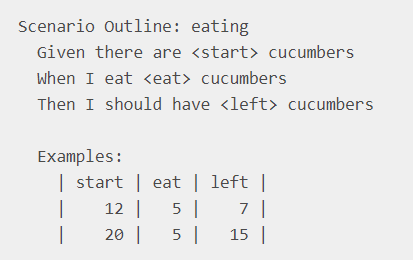
\includegraphics[width=\linewidth]{Scenario_outline.png}
		\caption{An example of a scenario outline}
		\label{fig15}
	\end{figure}
\end{itemize}

I. Bajwa, M. Naveed and M. Choudhary et al. have discussed the complexities in generating code from text descriptions \cite{e1}. They have compiled their findings under these categories:

\begin{enumerate}
	\item \textbf{Lexical Ambiguity}:
	Lexical ambiguity is created when a same word assumes various meanings \cite{e2}. In this case that ambiguity is generated from the fact that which meanings will be incorporated in which scenario. For instance, the word "bright" can be used in the following contexts,
	"The sun is bright."
	"That kid is very bright."
	It turns out obvious that the same adjective "bright" assumes two different meanings in the two sentences. In the first sentence it indicates the luminosity, and in the second, a quality of a person.
	
	\item \textbf{Syntactic ambiguities}:
	The syntax of a sentence can have huge implications on the meaning of that instance. For example, take the sentences, "eat me" and "me eat". A simple mistake within the syntax can completely muddle the meaning.
	
	\item \textbf{Semantic ambiguities}:
	Semantic analysis gives a sentence its meaning. Semantic ambiguities are most common due to the fact that generally a computer is not in a position to distinguish the
	logical situations. "The car hit the pole while it was moving." All of us would surely interpret the phrase like "The car, while moving, hit the pole.", while someone unused to reality might interpret it as, "the car hit the pole while the pole was moving " \cite{e1}. 
	
	\item \textbf{Pragmatic ambiguities}:
	Pragmatic ambiguities born when the communication happens between two persons who do not share the same context. In the following example, "I will arrive to the airport at 12 o'clock." In this example, if the addressed person belongs to a different timezone, the meanings can be totally changed. 
	 	 
\end{enumerate}

I expect that we do not encounter much in the way of lexical ambiguity as we have a limited set of domain and programming language specific terms to work with. This goes for syntactic ambiguities as well because there is little syntactic diversity in our scenario. But, this can arise in the case where there is a mistake in the Gherkin test case. To avoid these pitfalls, we can use more complex NLP processing. But, giving the user the last say in what the text means through the User Interface is the best safety check we can have, in my opinion.

The NLP processing of the Gherkin test cases must preserve the relationships between the entities when generating the output. Since the test case is broken into sections by the Gherkin keywords, we can first split the processing along this separation first. Then given such a statement, we have to break it to possible class, method and value attributes and tag them as such. Then the "Entity Relationship Extractor" can attempt to match them  with the existing code base.

 \subsection{Language Decider}
The language decider looks at the code base and decides what the target language is for the test case generation. Then, it loads the corresponding language modules in the Entity Graph Generator and Test Case Generator modules. Here, we assume that \textit{the code base provided is written in a single programming language.} So therefore, it is sufficient to look at a minimal number of code files to decide the target language. The ideal number of files would be 1 and hereafter, if not mentioned otherwise, we will consider that the Language Decider takes only 1 code file to determine the target language.
 
\subsection{Entity Graph Generator}
This module is responsible for parsing the available code base and $3^{rd}$ party sources, and generating a relationship graph which includes all of the available classes, their methods, inheritance and association relationships. Also, this module must include the classes, interfaces and methods form the base language. This is created for the use in the "Entity Relationship Extractor". The complexity here is that we are targeting multiple languages. There are two approaches we can take.

\begin{itemize}
	\item Implementing a system to identify the code from several languages. Here, we will have a module for each target language. In this approach, we have to code the module to understand all of the target language's linguistics and thus generate the relationship graph. It takes a considerable amount of coding on our part to handle all of the requisite languages.
	\item Using a neural network based solution. We can have multiple networks for each of the languages. But, in this solution, we need to have enough test scenarios of code and their graph representations to train the network.
\end{itemize}

We can organize the entity graph generators for the different languages as separate libraries, so they can be loaded at runtime, based on the analysis of the language decider. The entity Graph Generator must run at the first run of the process to scan the whole code base and generate the graph. This graph can be saved for future reference. Afterwards, whenever a change occurs in the code base, during the next run, the Entity Graph Generator must be able to discern that a change has occurred and accordingly modify the tree structure. So, this module must be capable of tracking the last modified time code of the existing files and recognizing the new additions to the code base. Also, in addition to that, the file entry should have entries of all the entity entries it contains. This is so that we can modify the entities in the graph when the files they are contained in are edited. Also, the entity entries must have references to their files for the purposes of inclusion. The graph should also allow the Entity Relationship Extractor module to access all of the elements in the graph structure.\newline
So we have discovered these relationships that must be included in the Entity Graph, in summary which are,
\begin{itemize}
	\item Time codes for all code base files.
	\item Entities included in each file.
	\item A file entry in each entity. (For file inclusion)
\end{itemize}

\subsection{Entity Relationship Extractor}
This section takes in the outputs of the previous two sections and tries to map the test case's entities to the entities from the code base graph. A NLP based difference checking between the entities in the test case and the entities in the code base graph. The major problem faced here is how to search for a specific keyword within the entity relationship graph. The solution we shall suggest is a tiered search. The search will start from the module to which the test case belongs. Then it will move to search the other directories.
We need a similarity measure to decide if there is a match between the BDD entity and the source code entities. Such measures can be,

\begin{enumerate}
	\item \textbf{A string matcher:} A simple string matcher that matches the class, method names using basic string operations.
	\item \textbf{An NLP matcher:} A matcher that considers the similarity between the two strings by considering the real life language meanings.
	\item \textbf{A context based matcher:} A matcher that attempts to match the entities based on descriptions and other relationships contained in the test case.
\end{enumerate}
 We opt to choose the last option as it provides the best opportunities for matching. The overall cost of operation for the module will be higher in this case than others and will take longer to find the final result.\newline
 Also, we will have to verify the decisions we have come up with the users. This is essential to avoid false positives in our search process. Therefore, this module must implement a GUI interface for the clients to interact with the program. The GUI should query the user when there are multiple possible matches or when there appears to be no matching entities to use. The user must be capable of manually resolving these problems. But, our goal is, given that the user, (or rather, the programmer who wrote the code) has followed standard accepted design principles, there will be no need for such disambiguation.\newline
 Once we have decide on the entities required to generate the test case, we shall pass the details learned to the test case generator.
 
\subsection{User Interface}
User Interface in our system has a several responsibilities.
\begin{enumerate}
	\item At the initial run, specify the code base root directory. Therefore, the code base must be contained within a single master directory.
	\item The UI must allow the user to specify the source directories of $3^{rd}$ party libraries.
	\item When generating the test, if there are multiple possible entities matching an entity in the Gherkin test case, the interface must ask the user to disambiguate.
	\item If there are no matching entities for an entity in the test case, the user interface must ask the user to browse to the entity's path if it exists and give path to save a stub generated by our system. 
	\item Refresh functionality must be available for the user to refresh the entity graph and other related data structures. Otherwise, the  graphs will be update them at startup.
	\item When generating the test glue code, the UI must prompt the user to inspect the generated code.
	
\end{enumerate}

\subsection{Test Code Generator}
The Test Code Generator will generate the test case based on the output of the Entity Relationship Extractor. The Entity Relationship Extractor feeds all the necessary code elements to the generator and the generator simply arranges them according to the target programming language's linguistics. To achieve this, we plan to use a GAN, whose generative network will act as the test code generator at the end of the training process.

\subsubsection{The Generative Network}
The generative network is responsible for the generation of the BDD style test cases based on the client requirements. This network requires natural language processing capabilities that can reliably process the client requirement, such that, this module must be capable of going through the requirement and deciding the necessary classes, methods and their signatures. Also, since the test is specified in the Gherkin style, this module must be capable of determining the control flow of the test as well. Now, after refining the architecture, we see that we can separate the initial language processing away from the neural network itself.\newline
This generative network is responsible for taking the output of the Entity Relationship Extractor and from it, generating the actual test, in the target programming language. The output of the Entity Relationship Extractor is not programming language specific. This is due to the fact that, we would like the output to be language agnostic so that we can use the output to generate code for multiple languages. As a result, we can have multiple code generation modules that can be used to generate code in multiple languages. As a result, we can have code generation modules for generating code for Java, C++, Python, JavaScript, etc. and thus we can support multiple code generation modules rather than a single code generation module. The Language Decider is responsible for loading the correct code generation module for the target code base. Such a setup is useful if we have code bases in multiple programming languages, as it is sometimes practiced in organizations to have code bases in different languages.

\begin{figure}
	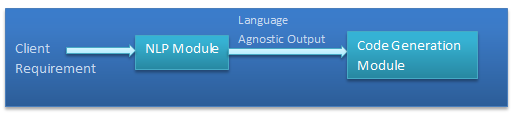
\includegraphics[width=\linewidth]{Gen_net_modules.png}
	\caption{Generative network modules}
	\label{fig7}
\end{figure} 

\begin{figure}
	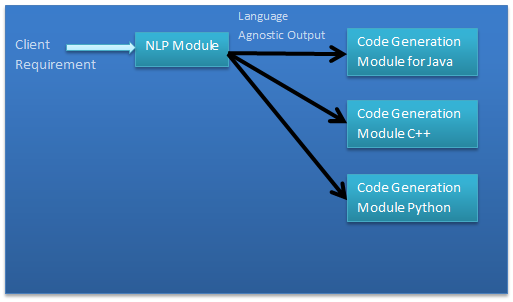
\includegraphics[width=\linewidth]{Gen_net_modules_multiple.png}
	\caption{Generative network modules with support for multiple languages}
	\label{fig8}
\end{figure} 

\subsubsection{The Discriminative Network}

The discriminative network will decide whether the output of the code generation module is valid. This can be done in two ways.

\begin{enumerate}
	\item\textit{Code consistency checking} : Checking whether the generated code is consistent with the rules of the target programming language.
	\item\textit{Consistency with client requirement} : This is checking whether the generated code is consistent with the client requirement. It involves NLP. 	
\end{enumerate}

Both of these are not programming language agnostic as the output of the code generation module is programming language specific. So if we need to support multiple languages, we will need multiple verification modules. Also it is advisable to have two modules to perform the aforementioned two tasks, with a module for each checking case. The complete validation module, thus achieved, is presented in the Fig. 27.\newline
The results from the verification modules are fed back to the generative modules to improve upon their generative process, so that as time goes on, the generative procedure will improve tot the point that the verification module will not distinguish between the actual valid cases and the generated cases that are fed to it.\newline
The code only verification module of the validation module set acts as the basic sanity test the generative network has to pass. Actually, we can first train with the code only verification module as the sole component of the discriminative network and then after it is satisfied, move onto the code and client requirement cross validation module. For the current project, we shall only be focusing on having a code consistency checking network. The full discriminative network with the code and client requirement consistency checking will be left as future work, since checking against the client requirement is not an immediate necessity for the discriminative network.

\begin{figure}
	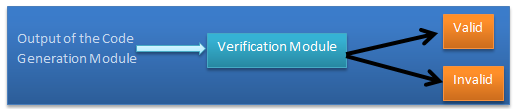
\includegraphics[width=\linewidth]{Validation_module.png}
	\caption{The basic validation module}
	\label{fig9}
\end{figure} 

\begin{figure}
	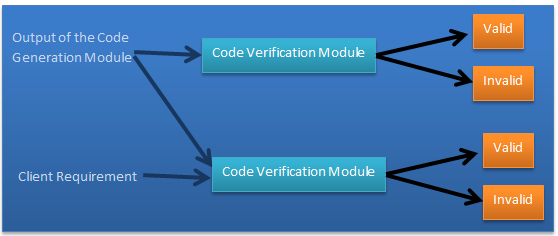
\includegraphics[width=\linewidth]{Complete_verification_module.png}
	\caption{The complete validation module set}
	\label{fig10}
\end{figure}

I would like to point out that we can replace this discriminative network with language syntax checkers. If so, like it was mentioned before, we would have to implement syntax checkers for each of our supported languages.

\subsubsection{Training}
For the training of the GAN, we can use one of two strategies for generating the input,
\begin{enumerate}
	\item Client requirements processed through the Token Extractor, along with simulated Entity Graph Generator outputs sent through the Entity Relationship Extractor.
	\item A simulation of the output of the Entity Relationship Extractor.
\end{enumerate}
We have to provide the proper test cases that implement the client requirements in our desired language along with these inputs as targets. Here, a single language is specified because we would have to train separately to support for multiple languages. Here we would only consider the case where a single programming language is present.\newline
The classes and methods that are available to generate the tests, i.e. the contents of the code base, will be filtered and only the relevant entities will be passed into the network for training. These can be existing code elements or code stubs generated by the Entity Relationship Extractor. The Discriminative Network needs to be trained to discern whether the generated test cases are consistent with the syntax of the programming language. We will train multiple generative and discriminative networks, each for a specific programming language. Apart from the developer created classes, the GAN must also learn to handle the basic data types of the language such as int, float, etc. and language provided data structures such as vectors, arrays, maps, etc. This is further more complicated when the developers use $3^{rd}$ party libraries, as we have to train for their specifics as well. So as to simplify matters, the first iteration can cover a subset of tests that are lower in complexity.\newline
The discriminative model is trained via feeding the valid test cases as input to the verification module (That discriminates between valid and invalid test case as far as programming language consistency is concerned. i.e. the code only verification module) as valid inputs and feeding invalid test cases as invalid inputs. This will train the discriminative network to distinguish between the valid and invalid test cases.\newline

\begin{figure}
	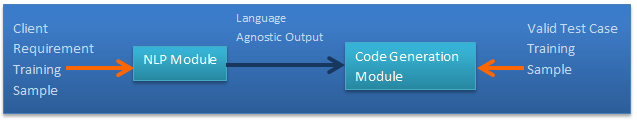
\includegraphics[width=\linewidth]{Generative_model_training.png}
	\caption{Generative model training plan}
	\label{fig11}
\end{figure} 

\begin{figure}
	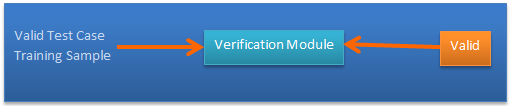
\includegraphics[width=\linewidth]{Discriminative_model_training.png}
	\caption{Discriminative model valid instance training plan}
	\label{fig12}
\end{figure} 

\begin{figure}
	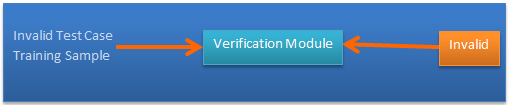
\includegraphics[width=\linewidth]{Validation_module_negative.png}
	\caption{Discriminative model invalid instance training plan}
	\label{fig13}
\end{figure} 

\subsubsection{After training}
After the training is completed, the only network we truly want is the generative network. Therefore, we are free to remove the discriminative network from the system when the training has been completed.

\subsection{Plan for operating the system}
The system is intended to function as a standalone application with a User Interface. First, the application is provided the root of the code base. Then the system recursively finds and maps all the classes and the public methods and members of the classes for the use of the Entity Relationship Extractor. The system will take some time to process the code base with the Entity Graph Generator and to generate the entity relationship graph. In the figure, "An abstract model of the entity relationship graph", you can see the basic idea of the entity relationship graph. Along with the relationship graph, the module also generates a hash keys-to-file path hash map so, fast lookups to entities can be facilitated.

\begin{figure}
	\centering
	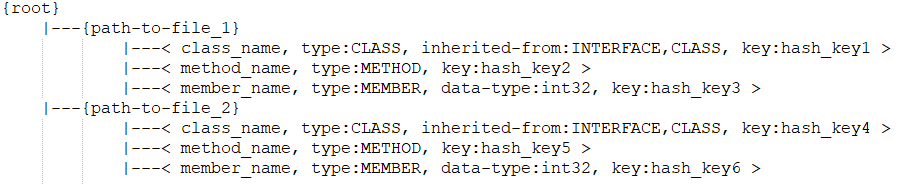
\includegraphics[width=0.7\linewidth]{graph_data_structure}
	\caption{An abstract model of the entity relationship graph data}
	\label{fig:graphdatastructure}
\end{figure}

The user can specify the root directory of the code base. Then our system recursively finds all the files belonging to the code base. Additionally, the user can provide the $3^{rd}$ party library source folder roots, so we can incorporate them into the code generation as well. The user also has to provide the test case specifications written in Gherkin as well. These can be provided one at a time or as a batch via a folder. Then the user can select to generate the glue code. Then our system will generate the glue code based on the data available. When generating code, if the system is unsure if an entity it has decided to use is the best, or if it needs to break a tie among several possible candidates, it must prompt the user to make the decision for it. Also, if the system deems necessary code is missing, it must provide the user with the option of either letting the system generate code stubs or if the code actually exists and our system failed to find it, browse to the position of the code file. Finally, before the code is generated, it must be presented to the user for review and modification.

\subsection{Difference between our system and Kirby}
The \textit{Kirby} system, which is an existing glue code generation solution for Java developers is very similar to what we are creating here in our project. But there are several dissimilarities between our project and \textit{Kirby}. They are,
\begin{enumerate}
	\item \textit{Kirby} only supports Java. Our system supports multiple programming languages.
	\item \textit{Kirby} is a plugin for the eclipse ide. Therefore, it cannot be used without the eclipse ide. Our system is a standalone application.
	\item Our system is a neural network based solution. \textit{Kirby} is not.
	\item \textit{Kirby} allows the user to also run the test cases and see their result. Our system currently does not support this.
\end{enumerate}

\section{Conclusions}
In the modern software development ecosystem it is imperative to deliver high quality software products to the clients efficiently. TDD and lately, BDD have helped tremendously to achieve these goals. The problem of generating test cases for user specified scenarios with awareness of the existing code base is a novel and a promising one which can help organizations and individuals to develop better code. Here we have outlined a proposal for generating BDD test cases automatically. We do not have to specify a target language for the test cases, as we can allow for the system to discover that on its own.

\begin{thebibliography}{00}
\bibitem{a1} Docs.cucumber.io. (2018). Gherkin Reference : Cucumber. [online] Available at: https://docs.cucumber.io/gherkin/reference/ [Accessed 22 Nov. 2018].
\bibitem{a2} Sunil Kamalakar, "Automatically Generating Tests from Natural Language Descriptions of Software Behavior" \textit{Thesis submitted to the Faculty of the
	Virginia Polytechnic Institute and State University
}
\bibitem{a3}Kelvin, A. (2017). "Source Code Generation from User Intention by Using Recurrent Neural Networks". [Blog] LinkedIn. Available at: https://www.linkedin.com/pulse/source-code-generation-from-user-intention-using-recurrent-kelvin/ [Accessed 19 Nov. 2018].
\bibitem{a4} Toshihiro Kamiya , Shinji Kusumoto , Katsuro Inoue, "CCFinder: a multilinguistic token-based code clone detection system for large scale source code", IEEE Transactions on Software Engineering, v.28 n.7, p.654-670, July 2002  [doi$>$10.1109/TSE.2002.1019480]
\bibitem{a5} L. Mou, R. Men, G. Li, L. Zhang, and Z. Jin. "On end-to-end program generation from user intention by deep neural networks." arXiv, 2015.
\bibitem{a6} H. Hy\"{o}tyniemi. Turing machines are recurrent neural
networks. Proc. STeP, 1996.
\bibitem{a7} R. Pascanu, T. Mikolov, and Y. Bengio. "On the difficulty of training recurrent neural networks." arXiv preprint, 1211.5063, 2012.
\bibitem{a8} S. Hochreiter and J. Schmidhuber. "Long short-term memory." Neural Comput., 9(8):1735–1780, 1997.
\bibitem{a9} K. Cho, B. van Merri\"{e}nboer, D. Bahdanau, and Y. Bengio. "On the properties of neural machine translation: Encoder-decoder approaches." arXiv
preprint, 1409.1259, 2014.
\bibitem{a10} I. Sutskever, O. Vinyals, and Q. Le. "Sequence to
sequence learning with neural networks." In \textit{NIPS}, 2014.
\bibitem{a11} Karpathy, A. (2018). The Unreasonable Effectiveness of Recurrent Neural Networks. [Blog] Andrej Karpathy blog. Available at: https://karpathy.github.io/2015/05/21/rnn-effectiveness/ [Accessed 22 Nov. 2018].
\bibitem{a12} A. Karpathy, J. Johnson, and F. Li. "Visualizing and understanding recurrent networks." arXiv preprint, 1506.02078, 2015.
\bibitem{d1} A. Egbreghts, "A Literature Review of Behavior Driven Development using Grounded Theory", Pdfs.semanticscholar.org, 2018. [Online]. Available: https://pdfs.semanticscholar.org/4f03/ec0675d08cfd1ecdbaac3361a29d756
ce656.pdf. [Accessed: 25- Nov- 2018].
\bibitem{d2} D. North, "Introducing BDD", Dan North \& Associates, 2018. [Online]. Available: https://dannorth.net/introducing-bdd/. [Accessed: 25- Nov- 2018].
\bibitem{d3} D. North, "How to sell BDD to the business - $\mid$ SkillsCast $\mid$ 27th November 2009", Skillsmatter.com, 2018. [Online]. Available: https://skillsmatter.com/skillscasts/923-how-to-sell-bdd-to-the-business$\sharp$showModal?modal-signup-complete. [Accessed: 25- Nov- 2018].
\bibitem{d4} Solis, C., and Wang, X., 2011. "A Study of the Characteristics of Behaviour Driven Development." 37th EUROMICRO Conference on Software Engineering and
Advanced Applications. Oulu. 383-387. DOI=10.1109/SEAA.2011.76
\bibitem{d5} Lopez-Pellicer, F.J., Latre, M.Á., Nogueras-Iso, J., Javier Zarazaga-Soria, F., Barrera, J. 2014. "Behaviour-driven development applied to the conformance testing of
INSPIRE web services." Lecture Notes in Geoinformation and Cartography. 325-339. DOI=10.1007/978-3-319-03611-3\_19
\bibitem{d6} Evans, E. 2004. "Domain-driven design: tackling complexity in the heart of software." Addison-Wesley Professional.
\bibitem{d7} Sathawornwichit, C., and Hosono, S. 2012. "Consistency Reflection for Automatic Update of Testing Environment." IEEE Asia-Pacific Services Computing Conference.
Guilin. 335-340. DOI= 10.1109/APSCC.2012.49
\bibitem{d8} Diepenbeck, M., Soeken, M., Grobe, D., and Drechsler, R. 2013. "Towards automatic scenario generation from coverage information." In Proceedings of the 8th International Workshop on Automation of Software Test (AST '13). IEEE Press, Piscataway, NJ, USA, 82-88
\bibitem{d9} Bâillon, C., Bouchez-Mongardé, S., 2010. "Executable requirements in a safety-critical context with Ada", Ada User Journal, 31 (2), pp. 131-135
\bibitem{d10} Sathawornwichit, C., and Hosono, S. 2012. "Consistency Reflection for Automatic Update of Testing Environment. IEEE Asia-Pacific Services Computing Conference.
Guilin. 335-340. DOI= 10.1109/APSCC.2012.49
\bibitem{b6}Siniaalto, Maria \& Abrahamsson, Pekka. "A Comparative Case Study on the Impact of Test-Driven Development on Program Design and Test Coverage". ESEM.2007., 2007, pp. 275 - 284.
\bibitem{e1} I. Bajwa, M. Naveed and M. Choudhary, "Natural Language Processing based Automatic Multilingual Code Generation", Pdfs.semanticscholar.org, 2018. [Online]. Available: https://pdfs.semanticscholar.org/fee0/d42fb08ef1618dadd83734bea38e
7b213f25.pdf. [Accessed: 26- Nov- 2018].
\bibitem{e2} Blaschke,C., Andrade,M.A., Ouzounis,C. and Valencia,A. (1999) Automatic extraction of biological information from scientific text: protein–protein interactions. Ismb, 60–67. 
\bibitem{b7}Beck, K., "Test-Driven Development By Example", AddisonWesley,
Boston, MA, USA, 2003.
\bibitem{b8}Astels, D., "Test-Driven Development: A Practical Guide",
Prentice Hall, Upper Saddle River, New Jersey, USA, 2003.
\bibitem{b9}Beck, K., Extreme Programming Explained, Second Edition:Embrace Change, Addison-Wesley, Boston, MA, USA, 2004.
\bibitem{b10}G. Larman and V.R. Basili, "Iterative and Incremental Development: A Brief History", IEEE Computer 36(6), IEEE Computer Soc., Los Alamitos, CA, USA, 2003, pp. 47-56.
\bibitem{b11} K. Beck, "Aim, fire", IEEE Software 18(5), IEEE Computer
Soc., Los Alamitos, CA, USA, 2001, pp. 87-89.
\bibitem{b1} I. J. Goodfellow, J. Pouget-Abadie, M. Mirza, B. Xu, D. Warde-Farley, S. Ozair, A. C. Courville, and Y. Bengio, "Generative adversarial
nets." In Proceedings of NIPS, pages 2672–2680, 2014
\bibitem{b12}Stephens, M. and D. Rosenberg, "Extreme Programming
Refactored: The Case Against XP", Apress, Berkeley, CA, USA,
2003.
\bibitem{b13}Boehm, B. and R. Turner, "Balancing Agility and Discipline
- A Guide for the Perplexed", Addison-Wesley, Boston, MA,
USA, 2004.
\bibitem{c1}B. George, L. Williams, "An Initial Investigation of Test Driven Development in Industry", Proc. ACM Symp. Applied Computing, 2003.
\bibitem{c2}Bhat, T. and Nagappan, N., "Evaluating the efficacy of testdriven
development: industrial case studies." In ISESE '06, Rio
de Janeiro, Brazil, 2006.
\bibitem{b2} J. Gauthier. "Conditional generative adversarial nets for
convolutional face generation." \textit{Class Project for Stanford
CS231N: Convolutional Neural Networks for Visual Recognition,
Winter semester,} 2014(5):2, 2014.
\bibitem{b3}T. Kim, M. Cha, H. Kim, J. Lee, and J. Kim. "Learning to discover cross-domain relations with generative
adversarial networks." International Conference on Machine Learning, 2017.
\bibitem{b4} L. Williams, E. M. Maximilien and M. Vouk, "Test-driven development as a defect-reduction practice", 14th International Symposium on Software Reliability Engineering, 2003. ISSRE 2003., 2003, pp. 34-45.
doi: 10.1109/ISSRE.2003.1251029
\bibitem{b5} H. Zhang, T. Xu, H. Li, S. Zhang, X. Huang, X. Wang, and D. Metaxas,
"Stackgan: Text to photo-realistic image synthesis with stacked generative
adversarial networks," arXiv preprint arXiv:1612.03242, 2016.
\end{thebibliography}

\pagebreak

\begin{appendix}
	\listoffigures
\end{appendix}

\vspace{12pt}

\end{document}
